\documentclass[twocolumn]{article}
\usepackage[margin=0.2in]{geometry}
\usepackage{multicol}
\usepackage{graphicx} % Already includes graphics
\usepackage{wrapfig}
\usepackage{amsmath}
\usepackage{amssymb}
\usepackage{array}
\usepackage{gensymb}
\usepackage{booktabs}
\usepackage{subcaption}
\usepackage{hyperref}
\usepackage{caption} % for \captionof
\usepackage{xcolor}
\title{\textbf{Radioactivity}}
\author{Arshbir Singh}

\begin{document}

\maketitle
\begin{center}
\Large
\textbf{Abstract}

\end{center}
In this set of experiments, we discover the basic properties of elemental decay and radiation by using a Geiger–Müller tube provided along with an electronic counter connected to the computer via software, and discs of various radioactive isotopes (Sr-90, Cs-137, and Co-60) and liquid Ba-137m. The penetration/Absorption/Backscattering factors have also been observed by using plates of various materials and thickness. 

\begin{center}\section*{Background}\end{center}
\subsection*{Radiation}
$Radiation$, a term coined by Curie, and observed during the 1800s refers to the spontaneous emission of radiation by an unstable nucleus to lose energy in order to move to a more stable configuration. Too many neutrons in a nucleus lead it to emit a negative $beta$ particle, which changes one of the neutrons into a proton. Too much energy leads a nucleus to emit a $gamma$ ray, which discards energy without changing any of the particles in the nucleus. Too much mass leads a nucleus to emit an $alpha$ particle, discarding four heavy particles (two protons and two neutrons). So, in terms of energy $gamma$ rays come first, $beta$ second, and $alpha$ particles third. How do we measure it? It is measured in number of disintegrations per second ($dps$) with Becquerel ($Bq$) the $S.I.$ unit equal to 1 $dps$. We are constantly being showered in radiation, and the absorbed dose is usually measured in $Gray(Gy)$ but, in $c.g.s.$, it is Roentgen equivalent man ($rem$). We refer to this radiation as Background radiation, and will measure it in one of the experiments.\\

\begin{equation*}
1Bq=1dps
\end{equation*}

\begin{equation*}
1Ci=3..6\times10^{10} Bq
\end{equation*}

\begin{equation*}
1rad=0.01Gy
\end{equation*}

\begin{equation*}
1rem=0.01Sv
\end{equation*}


\subsection*{Geiger–Müller tube/counter}
The tube is the detecting element of the counter, and works on the principle of $Townsend$ $avalanche$ (after detecting a radiation signal) to amplify it to a detectable electronic signal processed by the counter which then, forwards it into the computer allowing us to analyze the data. The tube is the main part, and how it works is a beautiful concept. It is filled with an inert gas, and when radiation enters the tube, and hits the gas atoms, they get ionized. There is a high voltage applied across the center (tungsten electrode, there seems to be a transformer hidden inside s-360) and the edges of the tube so the ions rush to the respective sides.  The electrons can reach very speeds, and in turn ionize other atoms, and it starts a chain reaction called $Townsend$ $avalanche$ or $gas$ $multiplication$ which leads to a detectable signal. The electron also experiences deceleration and due to $Bremsstrahlung$, releases photons which can also ionize other atoms in various directions. So, it becomes very chaotic inside the tube. There is a period between when radiation first enters the tube, and when electrons finally complete the circuit across the counter. During this time, no other radiation can be detected. This time is called $dead$ $time$. 
\begin{center}
\begin{figure}[t!]
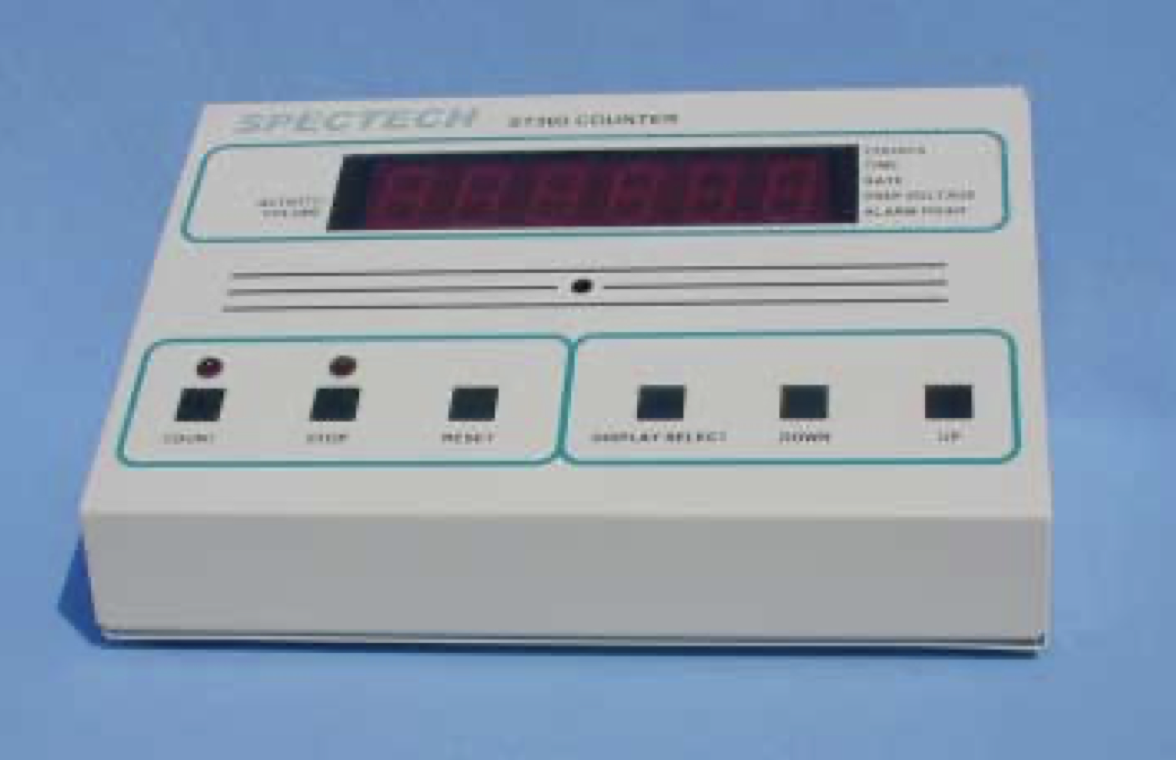
\includegraphics[scale=0.45]{counter.png}
\caption{Spectrum S-360 counter used in the experiments}
\end{figure}
\end{center}
\begin{center}
\begin{figure}[t!]
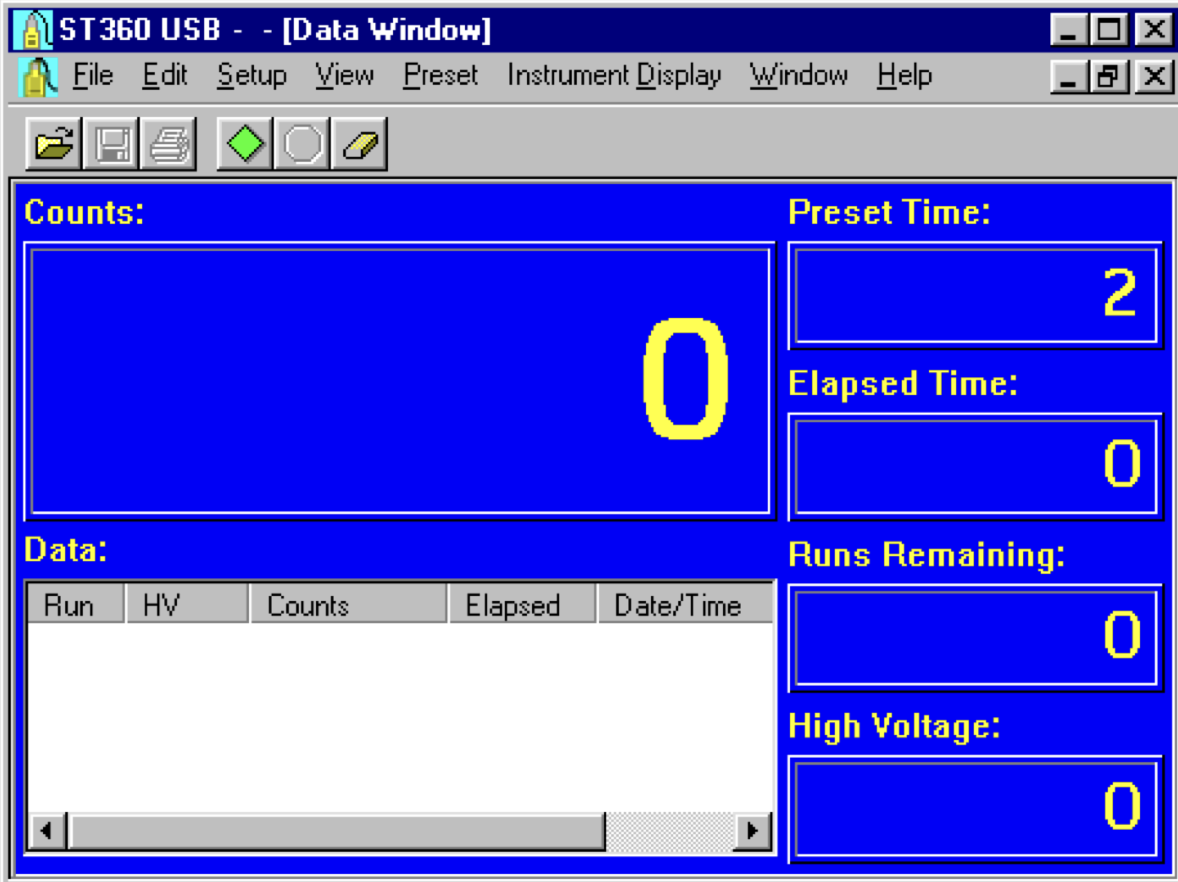
\includegraphics[scale=0.45]{screen.png}
\caption{example of the software interface used during the experiments.}
\end{figure}
\end{center}



%E1

\begin{center}\section*{\underline{Experiment 1: Plotting a GM Plateau}}\end{center}
\subsection*{Introduction}
All Geiger–Müller tubes have different operating voltages, and it doesn't start counting right away from zero voltage. There is a minimum threshold required for the avalanche to start, and hence, the signal to be detected. As, the voltage is increased even further, the counting rate increases until, at some maximum threshold value, it stabilizes. This point is called $knee$ $voltage$. The stabilization region looks like a plateau on the graph, and the last region where the plateau ends is called $discharge$ $region$. The first task is to find the optimal voltage by looking for the plateau. 
\subsection*{Procedure}
1. Assuming the counter (S-360) powered on, is connected to the PC, and ST360 interface running, we place a radioactive disc (Cs-137) on the tray under the tube.\\
\begin{center}
\begin{figure}[h!]
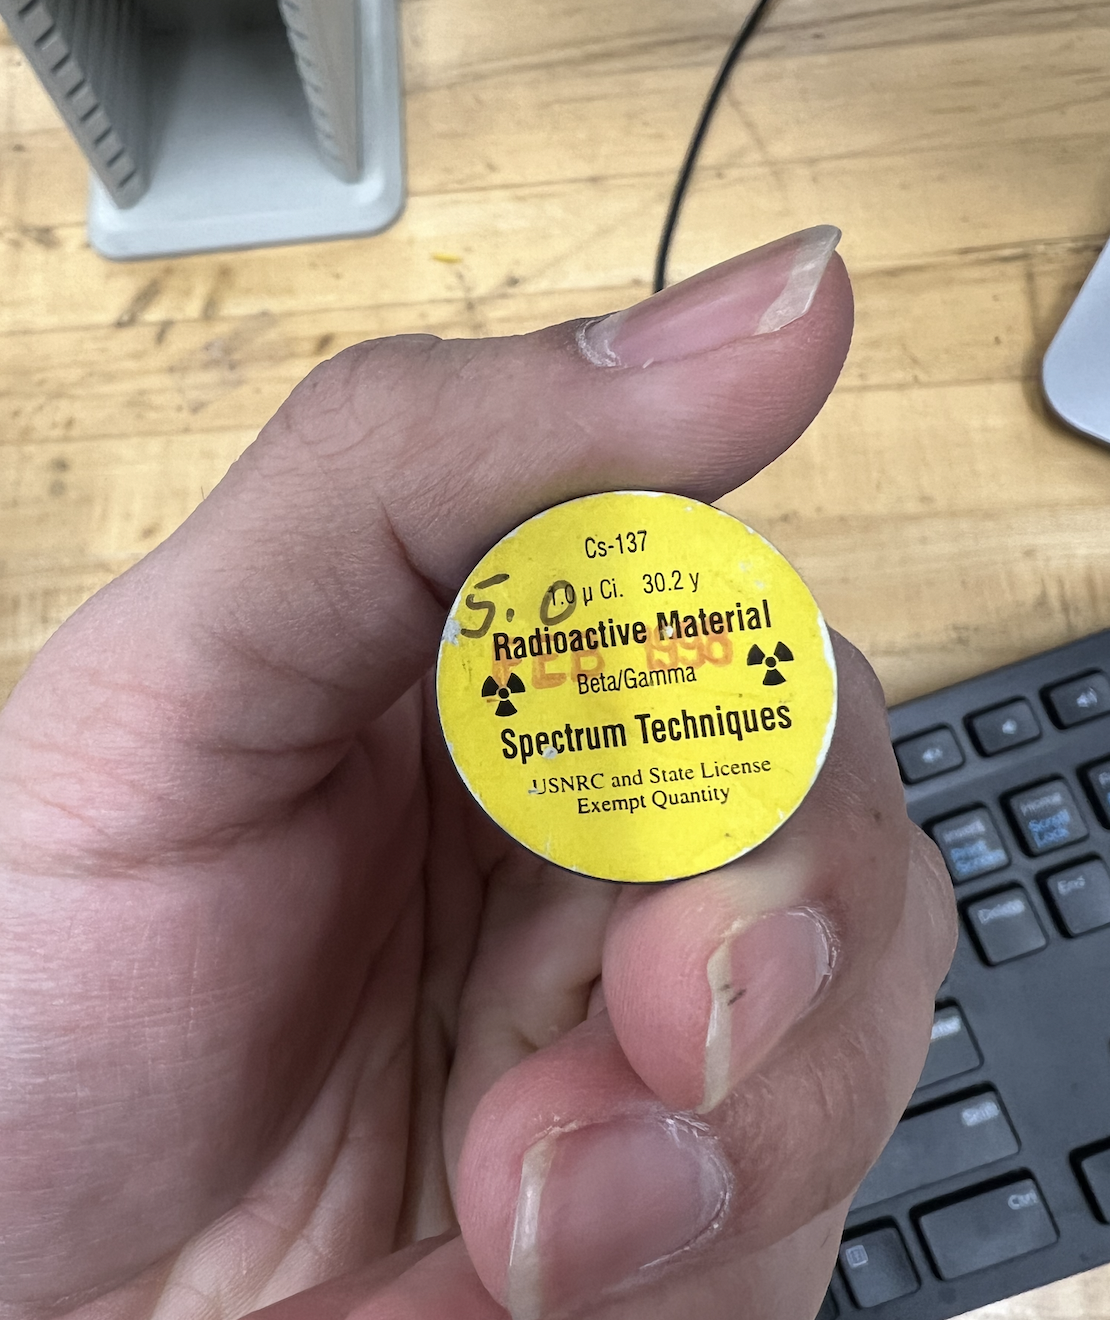
\includegraphics[scale=0.45]{disc.png}
\caption{Cs-137 disc we used in this experiment.}
\end{figure}
\end{center}
2. Next, we go to the \textbf{Setup} menu and select the \textbf{HV Setting} option. It automates the process for us. We started from 650 V with a step voltage of 50V all the way up to maximum possible 1200V.\\
3. Then, we select 30 seconds each run with 26 runs.\\
\subsection*{Inference}
 Counting starts at 700V. We can see in the graph below that there is indeed some kind of plateau but, we need to show it quantitatively. For that, we can refer to $slope(\%) $:
\begin{equation*}
Slope(\%)=\frac{100(R_2-R_1)}{R1(V_2-V_1)}\times 100
\end{equation*}

\begin{center}
\begin{figure}[h!]
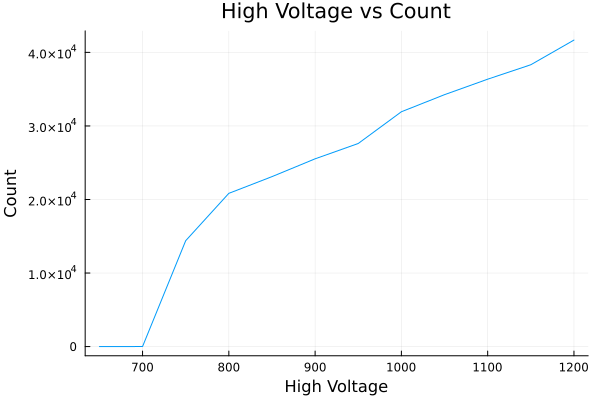
\includegraphics[scale=0.45]{lab1c.png}
\caption{We can see kind of a stabilization in the middle of the graph pointing to the presence of the plateau we were looking after.}
\end{figure}
\begin{figure}[h!]
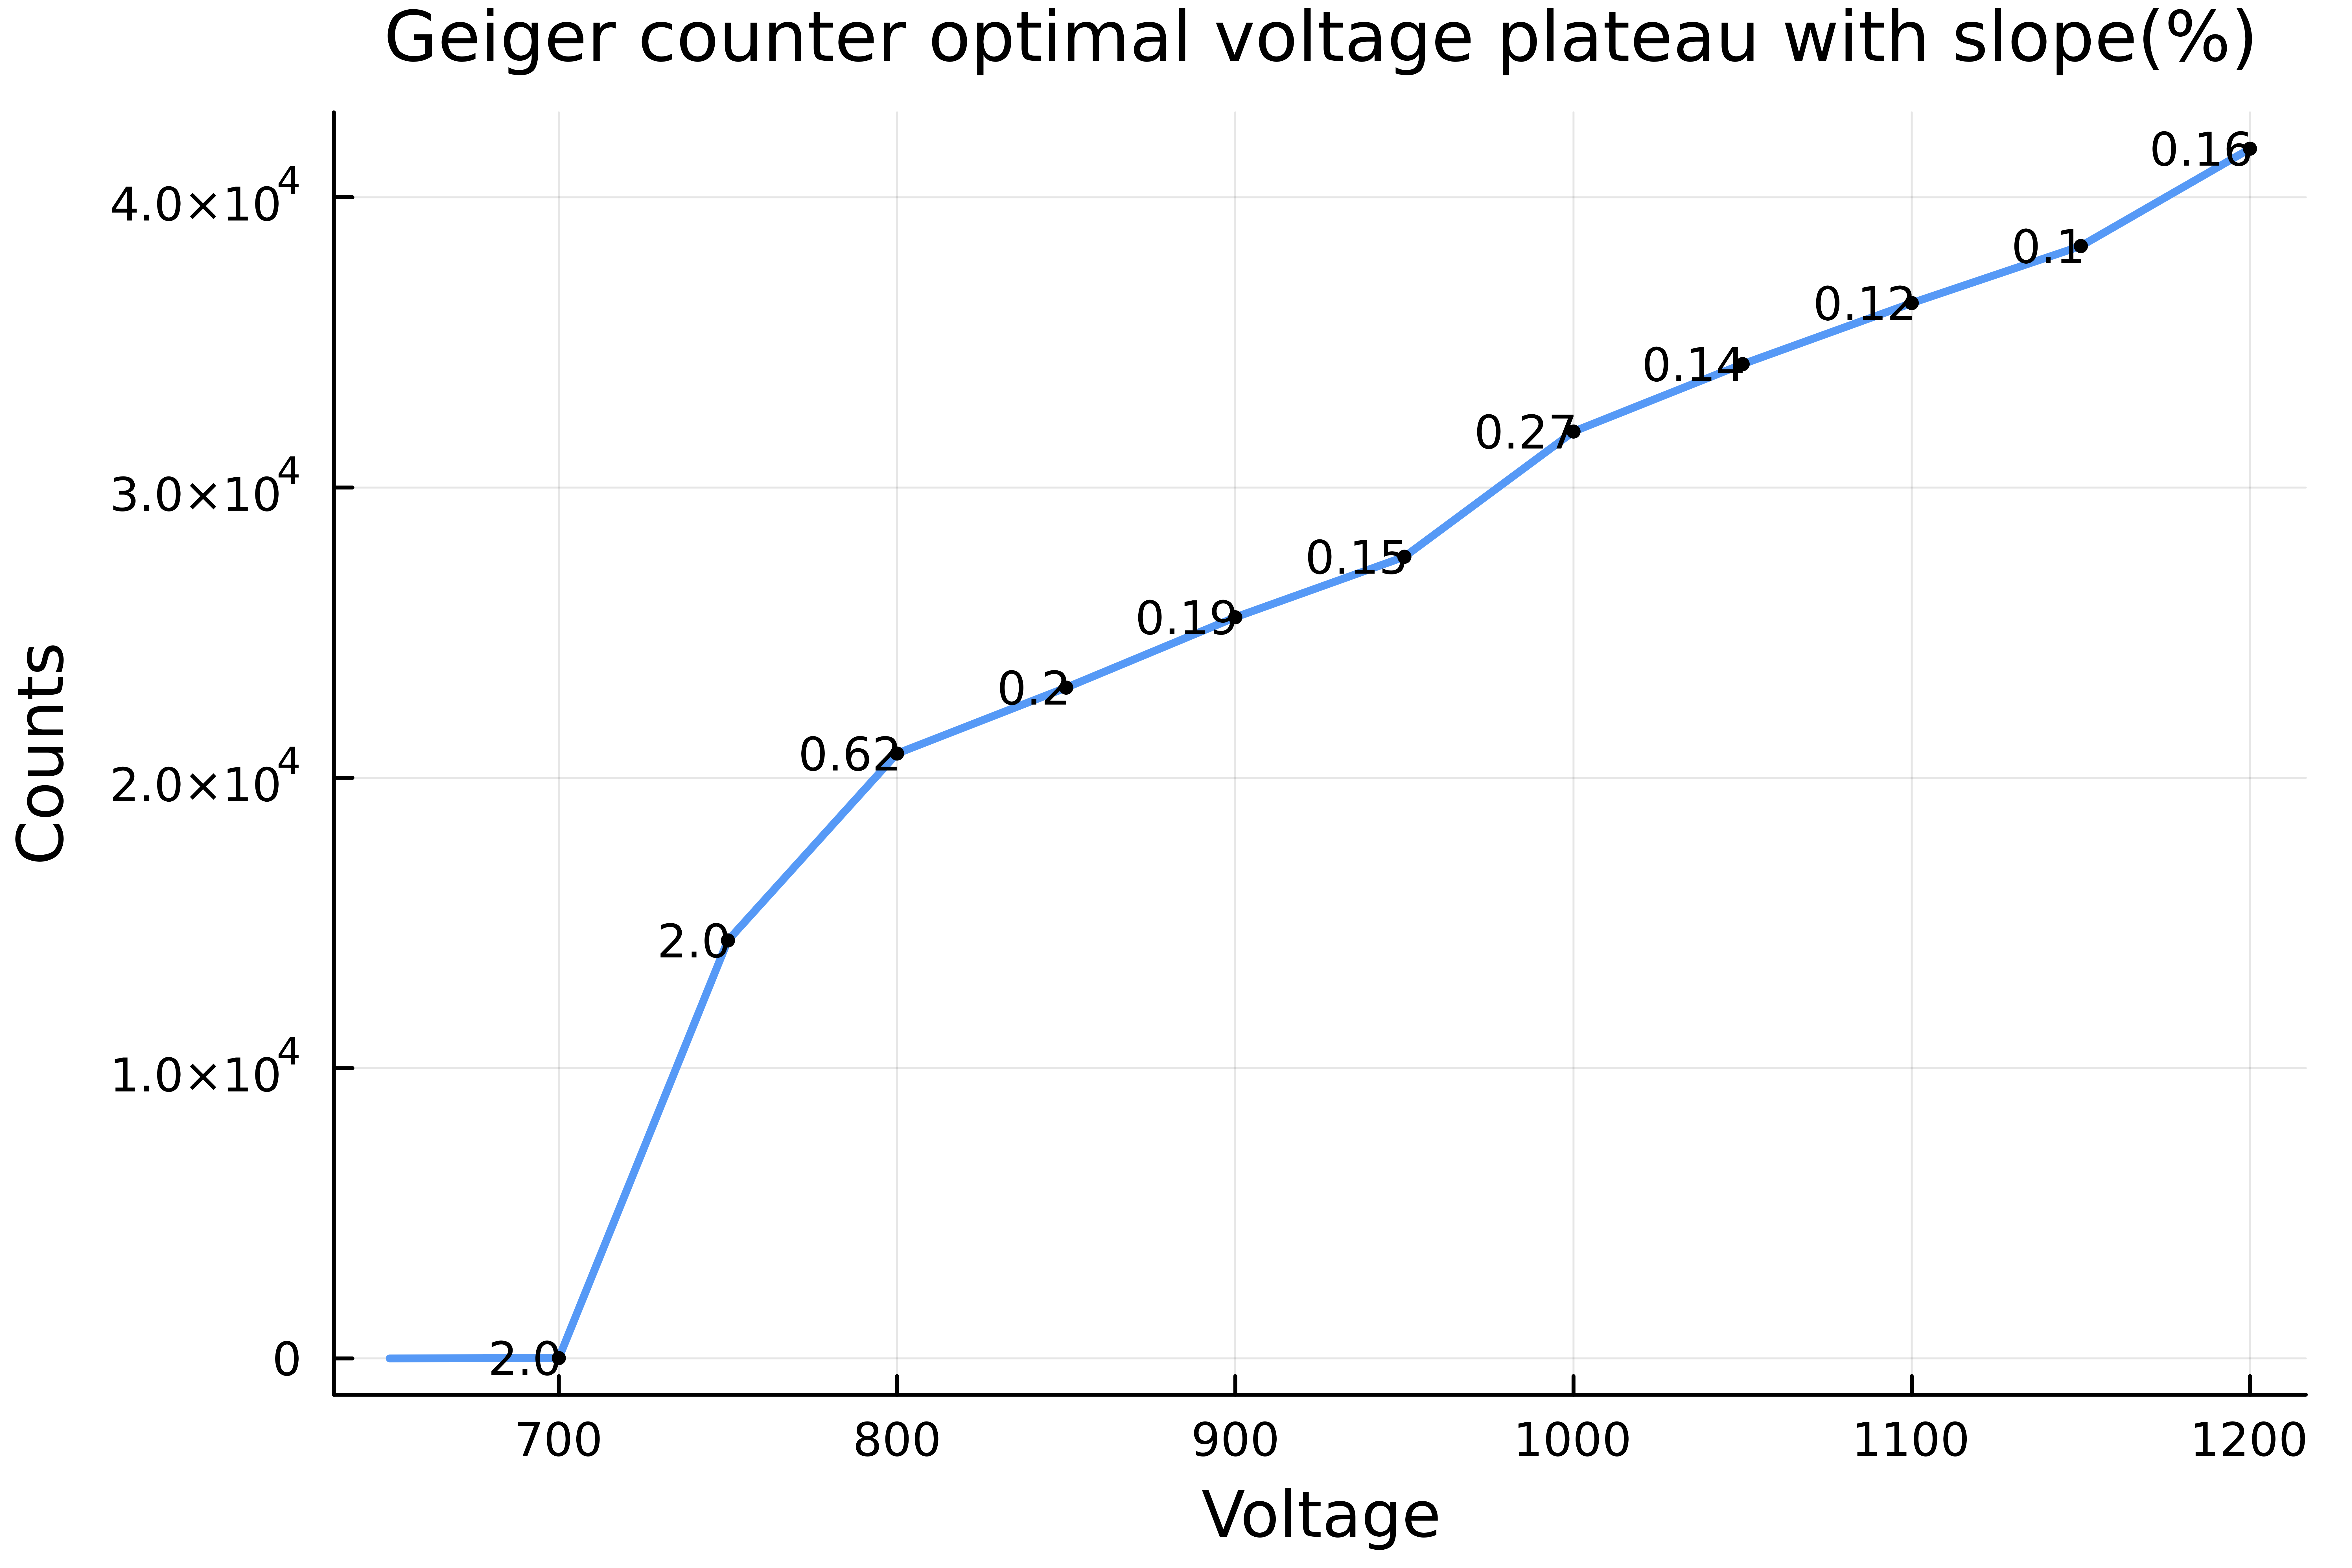
\includegraphics[scale=0.033]{lab10.png}
\caption{The slope percentage method for analyzing the plateau voltage}
\end{figure}
\end{center}
We can see in the second graph that the difference in slope percentage is lowest for the three values (0.2, 0.19, 0.15) at 850V, 900V, and 950V respectively. Therefore, 900V is the middle of the plateau, and hence the optimal operating voltage we've been looking after, and will use it in next experiments.\\


\begin{table}[h!]
  \centering
  \caption{Data Table for Geiger Plateau Lab}
  \begin{tabular}{|c|c|}
    \hline
    Voltage & Counts \\
    \hline
    650 & 0 \\
    \hline
    700 & 11 \\
    \hline
    750 & 14398 \\
    \hline
    800 & 20837 \\
    \hline
    850 & 23108 \\
    \hline
    900 & 25531 \\
    \hline
    950 & 27616 \\
    \hline
    1000 & 31929 \\
    \hline
    1050 & 34252 \\
    \hline
    1100 & 36356 \\
    \hline
    1150 & 38320 \\
    \hline
    1200 & 41674 \\
    \hline
  \end{tabular}
\end{table}








$$$$



%E2

\begin{center}\section*{\underline{Experiment 2: Statistics of Counting}}\end{center}
\subsection*{Introduction}
Due to a large number of simultaneous disintegrations, we turn to statistics to find any predictable patterns or suitable inferences. We'll be using Poisson($\lambda$) and Gaussian/Normal Distributions. The mean of a distribution ($\bar{x}$) can be formed as
\begin{equation*}
\bar{x} = \frac{1}{N} \sum_{i=1}^{N} x_i
\end{equation*}
and the standard deviation($\sigma$) shows how dispersed the values are relative to the mean, and can be found as
\begin{equation*}
\sigma = \sqrt{\frac{\sum_{i=1}^{N}(\bar{x}-x_i)^2}{N-1}}
\end{equation*}
To understand Poisson and Gaussian distributions, we need to start from binomial distributions. This is used when we have two outcomes. In a binomial distribution, say we have N objects,  let p be the probability of getting one of the outcomes(A), and q for B. p and q add up to 1. The probability that n out of N objects are in A is given by 
\begin{equation*}
P(n)=\frac{N!}{(N-n)!n!}p^nq^{N-n}
\end{equation*}
As we have seen, we're dealing with pretty high counts (N) with very small probabilities of success (p). Poisson distribution is just a special case of binomial distribution that satisfies those two conditions. For Poisson distribution
\begin{equation*}
P(n)=\frac{(Np)^n}{n!}e^{-(Np)}
\end{equation*}
where the mean of the distribution $(m)$ is given by 
\begin{equation*}
m=Np
\end{equation*}
and standard deviation for individual measurements by 
\begin{equation*}
\sigma=\sqrt{N}
\end{equation*}
For large values of $m$, Poisson distribution approaches the famous bell curve or Gaussian distribution given by 
\begin{equation*}
P(n)=\frac{1}{\sigma \sqrt{2\pi}}exp[-\frac{(x-m)^2}{2\sigma^2}]
\end{equation*}
with $m$ and $\sigma$ in the first lines. Note that Poisson distribution observes discrete values and cannot be negative. It is skewed to one side. On the other hand normal distribution is continuous and symmetric about the mean.
\subsection*{Pre-lab Questions}
1. List the formulas for finding the means and standard deviations for the Poisson and Gaussian distribution.\\
\textbf{Answer.} Given above.\\


2. A student in a previous class of the author’s once made the comment, “Why do we have to learn about errors? You should just buy good and accurate equipment.” How would you answer this student?\\
\textbf{Answer.} There isn't any equipment perfectly 100 percent accurate or precise, so it's helpful to learn and look for errors to account for uncertainties, and reasoning for them.

\subsection*{Procedure}
1. We set up the equipment as before, and set the voltage to 900V.\\
2. Then, we go to the preset menu setting the time to 5s and runs to 150.\\
3. First, we measure the background radiation.\\
3. Next, we repeat with Cs-137 with time per run equal to 1s, and runs to 750(the total time will be same as before).\\
\subsection*{Inference}
We have seen that for large N, the distribution is pretty much symmetric. As it should be, as we found the standard deviations in the Gaussian to be closer than Poisson. 
\begin{center}

\begin{figure}[h!]
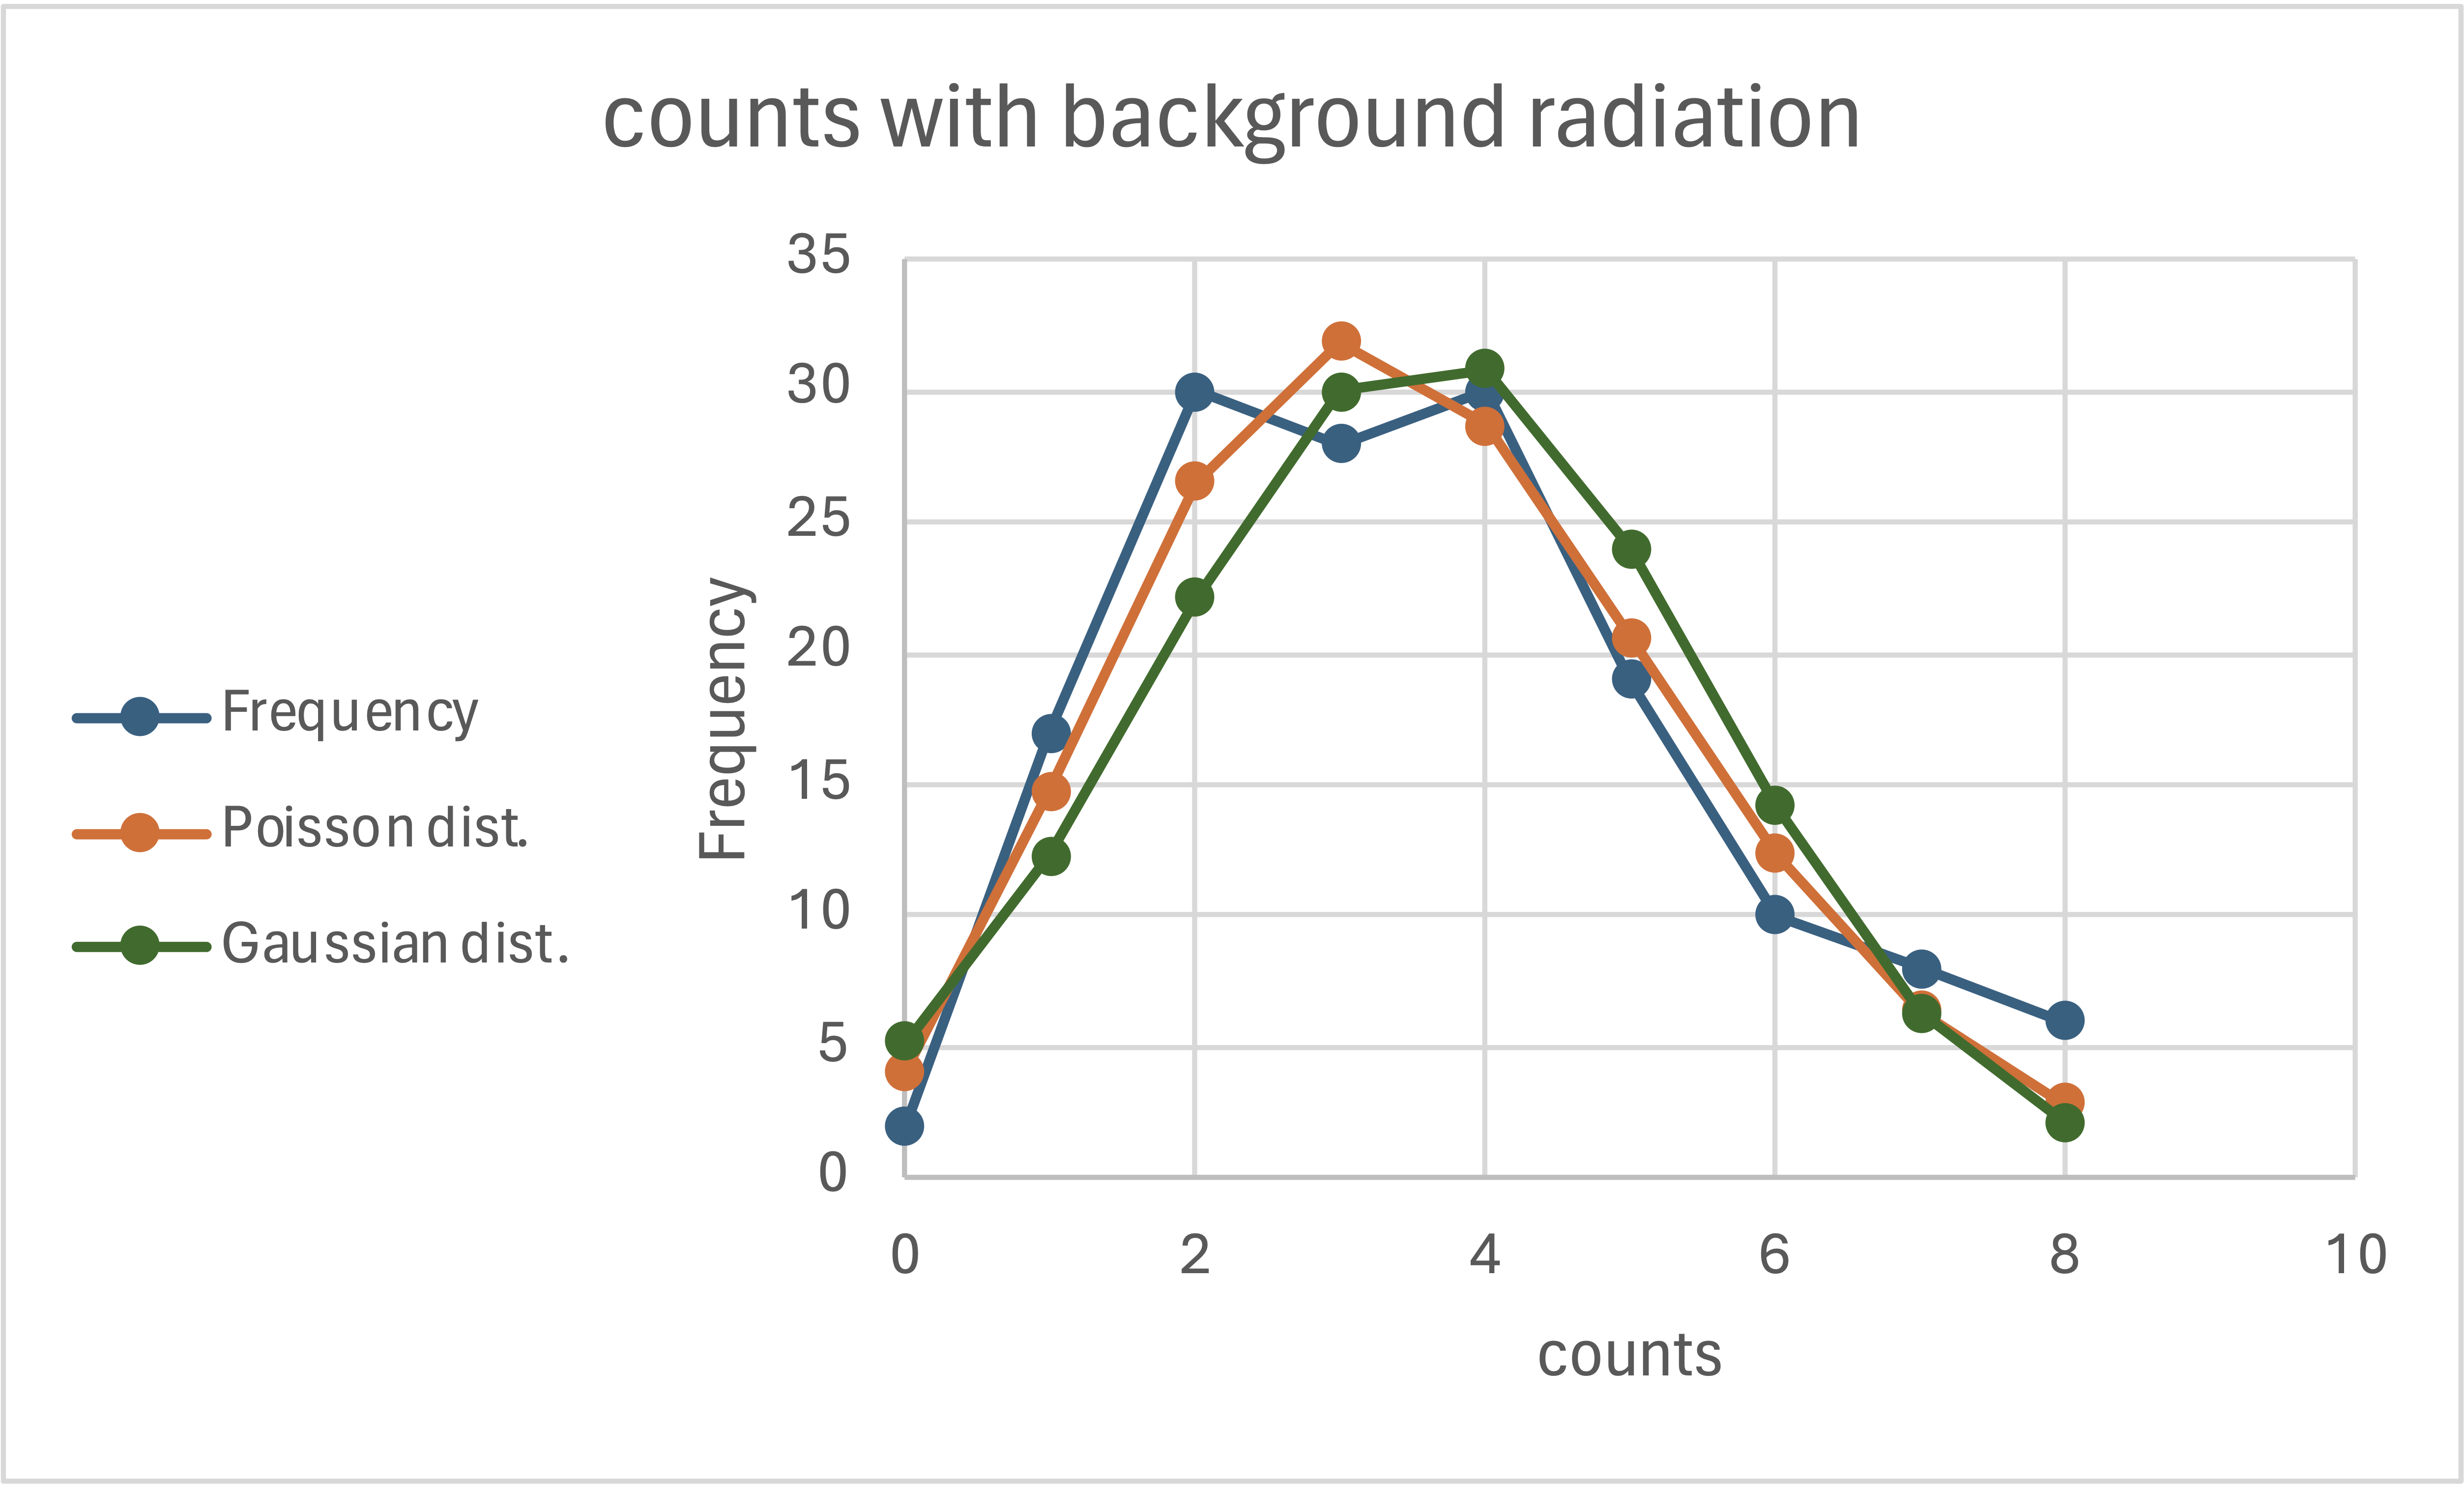
\includegraphics[scale=0.05]{lab2_a.png}
\caption{\small Frequency, Poisson, and Gaussian distribution for background radiation counts.}
\end{figure}
\begin{figure}[h!]
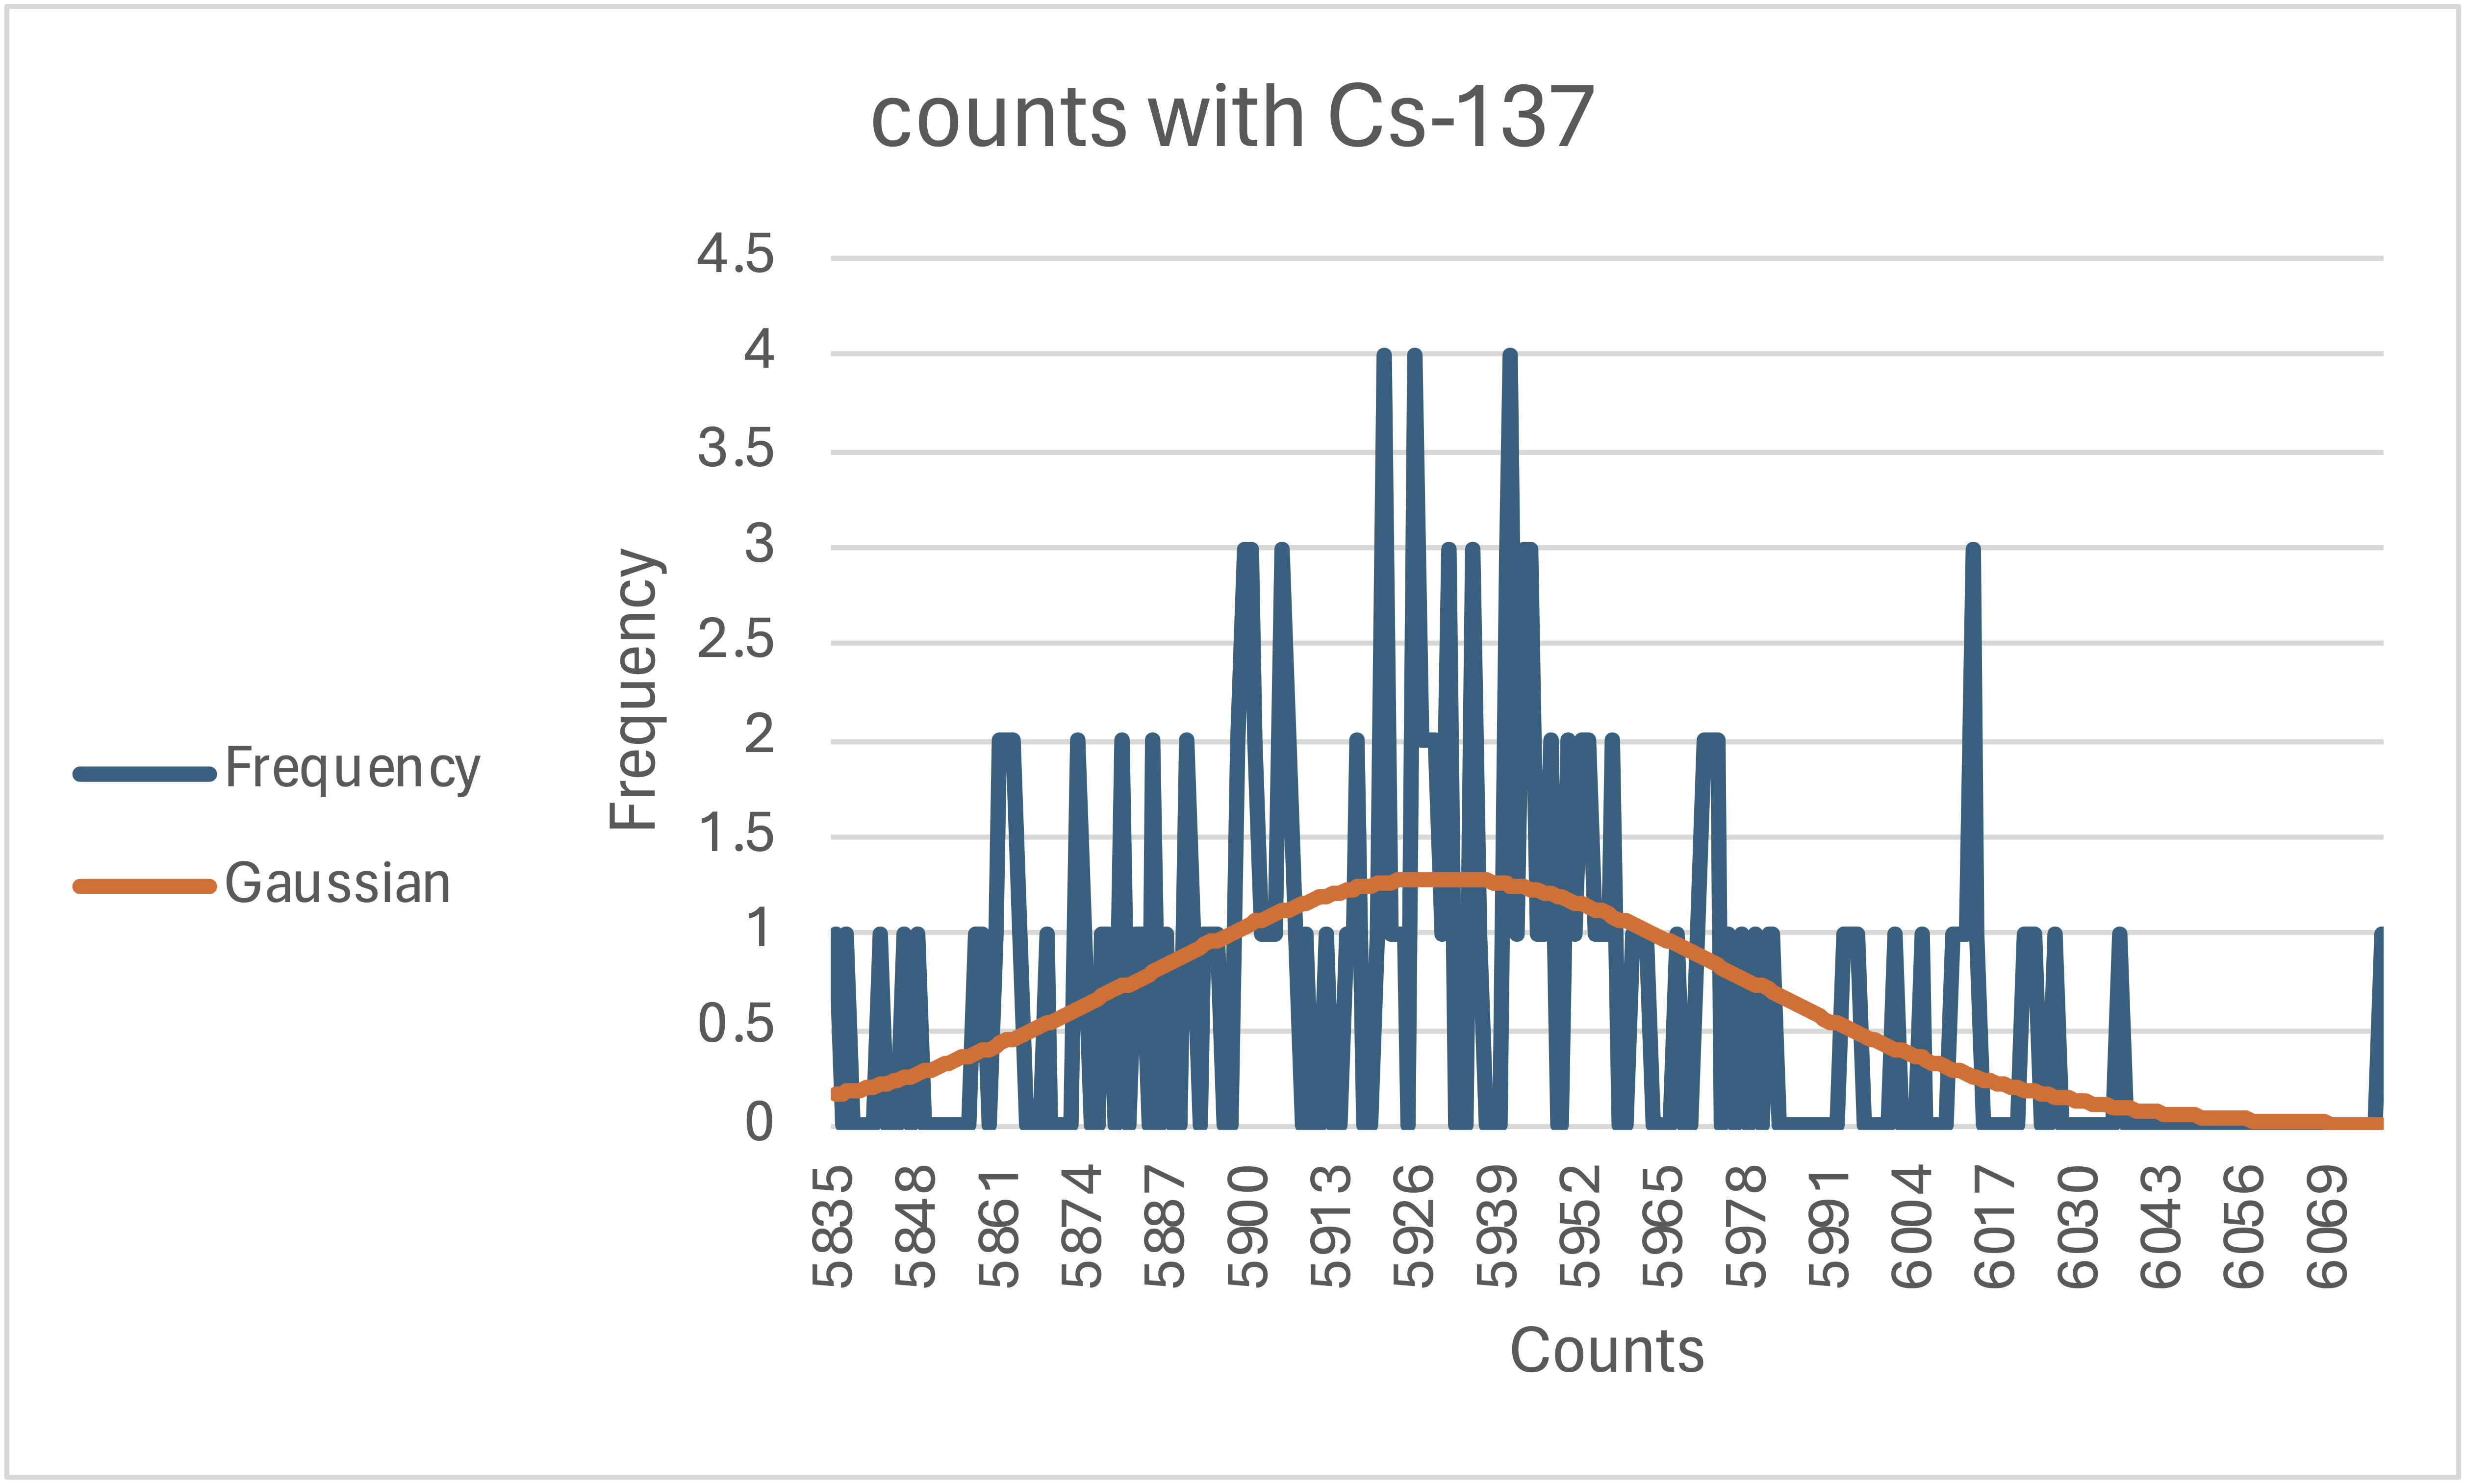
\includegraphics[scale=0.05]{lab2_b.png}
\caption{\small Frequency, and Gaussian distribution for Cs-137 disc counts. Note, there is no Poisson distribution due to large number of counts.}
\end{figure}
\end{center}



\begin{table}[h!]
  \centering
  \caption{counts with background radiation}
  \begin{tabular}{|c|c|c|c|}
    \hline
    Mean & 3.6\\
    \hline
    Minimum &0\\
    \hline
    Maximum&8\\
    \hline
    Standard Deviation&1.896659019\\
    \hline
    Square Root of Mean &1.897366596\\
    \hline
  \end{tabular}
\end{table}


\begin{table}[h!]
  \centering
  \caption{Statistics with background radiation. N goes from the minimum to the maximum counts in 5 seconds.}
  \begin{tabular}{|c|c|c|c|}
    \hline
    \textbf{N} & \textbf{Frequency} & \textbf{Poisson dist.$\sigma$} & \textbf{Gaussian dist.$\sigma$} \\
    \hline
    0 & 2 & 4.098558367 & 5.208331473 \\
    \hline
    1 & 17 & 14.75481012 & 12.3297283 \\
    \hline
    2 & 30 & 26.55865822 & 22.10451614 \\
    \hline
    3 & 28 & 31.87038986 & 30.01104618 \\
    \hline
    4 & 30 & 28.68335088 & 30.85701229 \\
    \hline
    5 & 19 & 20.65201263 & 24.02698227 \\
    \hline
    6 & 10 & 12.39120758 & 14.1682822 \\
    \hline
    7 & 8 & 6.37262104 & 6.327144965 \\
    \hline
    8 & 6 & 2.867679468 & 2.139789182 \\
    \hline
  \end{tabular}
\end{table}

\begin{table}[h!]
  \centering
  \caption{counts with Cs-137 disc as the source-radiation}
  \begin{tabular}{|c|c|c|c|}
    \hline
    Mean & 5930\\
    \hline
    Minimum &5835\\
    \hline
    Maximum&6077\\
    \hline
    Standard Deviation&46.55832742\\
    \hline
    Square Root of Mean &77.00649323\\
    \hline
  \end{tabular}
\end{table}
Again, there are 243 entries so, the table hasn't been listed but, the graph (shown on the left) is more appropriate for any analysis.\\
\subsection*{Post-lab Questions}
1. Which distribution matches the data with the background counts? How well does the Gaussian distribution describe the Cs-137 data?\\
\textbf{Answer.} Poisson distribution matches the data with the background counts. Gaussian distribution doesn't seem to describe the data well because of the visible fluctuations on the graph. \\
\\
2. Why can’t you get a value for the Poisson distribution with the data from the Cesium-137 source?\\
\textbf{Answer.} The standard deviation of the distribution depends on the half-life of the radioactive source used. Cs-137 has a comparatively long half-life (about 30 years). For values greater than 20, it becomes a Gaussian distribution. Therefore, we cannot get a value for the Poisson distribution with Cs-137.\\
\\
3. How close are the standard deviation values when calculated with the Poisson and Gaussian Distributions? Is one right (or more correct)? Is one easier to calculate?\\
\textbf{Answer.} The values are closer when calculated with the Gaussian Distribution with mean 16.31. Poisson is easier to calculate. However, Gaussian Distribution is more insightful because of large N and closer Standard deviations.\\ 









$$$$
%E3


\begin{center}\section*{\underline{Experiment 3: Background Radiation}}\end{center}
\subsection*{Introduction}
As we mentioned before, we're constantly being bombarded with radiation. When the count is low, this radiation can cause very high errors. Therefore, we must measure it, and use it to account for the errors in our calculations with any sources.
\subsection*{Pre-lab Questions}
1. Name the four natural sources and three man-made sources of background radiation.\\
\textbf{Answer.}\\ Four natural sources are:\\
a. CMBR/cosmic radiation\\
b. Terrestrial radiation is emitted by naturally occurring radioactive elements present in earth's core.\\
c. Pulsars are highly magnetized rotating neutron stars that emit beams of radiation along their magnetic axes.\\
d. AGN(Active Galactic Nuclei) emit radiation across the spectrum, including X-rays and gamma rays.\\
\\
Three man-made sources are:\\
a. medical equipment such as X-rays and CT scans,\\
b. WMDs\\
c. Nuclear power plants\\
$$$$ 
2. Approximately how much background radiation is received by an average American citizen every year? Is this very high (dangerous)?\\
\textbf{Answer.} 6.2 millisieverts or 620 millirem per person per year(EPA.gov). The current federal occupational limit of exposure per year for an adult (the limit for a worker using radiation) is "as low as reasonably achievable; however, not to exceed 5,000 millirems" (MIT). Therefore, it's relatively safe.

\subsection*{Procedure}
1. We set-up the counter as before, without any disc. The voltage is set to 900V.\\
2. We'll do 3 runs at 300s (5minutes) each. So, total 15 minutes.\\
3. Then, we repeat the same measurements but, with Cs-137 disc.\\
 \subsection*{Inference}
 \begin{table}[h!]
  \centering
  \caption{counts with background radiation}
  \begin{tabular}{|c|c|c|c|}
    \hline
    \textbf{Run Number} & \textbf{High Voltage} & \textbf{Counts} & \textbf{Elapsed Time} \\
    \hline
    1 & 900 & 197 & 300 \\
    \hline
    2 & 900 & 189 & 300 \\
    \hline
    3 & 900 & 184 & 300 \\
    \hline
  \end{tabular}
  
  
\end{table}
 \begin{table}[h!]
  \centering
  \caption{counts with Cs-137 disc as radiation source}
  \begin{tabular}{|c|c|c|c|}
    \hline
    \textbf{Run Number} & \textbf{High Voltage} & \textbf{Counts} & \textbf{Elapsed Time} \\
    \hline
    1 & 900 & 251738 & 300 \\
    \hline
    2 & 900 & 252382 & 300 \\
    \hline
    3 & 900 & 252399 & 300 \\
    \hline
  \end{tabular}
\end{table}
Corrected counts can be found using the difference after averaging out the three runs from both samples, and was found to be 251983 counts.
\subsection*{Post-lab Questions}
1. Is there anyway to eliminate background radiation?\\
\textbf{Answer.}We can try to move away from known radiation sources such as phones. Also, we can do shielding with lead plates which will be shown in one of the experiments.\\
2. What is your prediction for the number of background radiation counts that your body would receive a day? (Hint: convert from $cps$ or $cpm$ into $cpd$,
counts per day.) How many counts per year?\\
\textbf{Answer.} The average is 190 in 300 seconds so, \begin{equation*}
\frac{190\times60\times60\times24\times365}{300}\approx 1.99728\times 10^7
\end{equation*}
\\
3. Are all the background measurements exactly the same number of counts?
Is there a systematic cause for this?\\
They are definitely not the same because as mentioned earlier, there is some degree of randomness in radiation. Also, we can't go below dead count. Nonetheless, there is standard deviation of only 6.557438524, and they're pretty close by.
\\





$$$$
%E5

\begin{center}\section*{\underline{Experiment 5: Geiger Tube Efficiency}}\end{center}
\subsection*{Introduction}
We know GM tube does not count all the particles that are emitted from a source, i.e., dead time. In this experiment, we'll find the disintegration rate (activity) of the source. The conversion factor  $1\mu Ci=2.22\times 10^6 dpm$ will be useful. Also, \begin{equation*}
\% Efficiency=\frac{r(100)}{CK}\end{equation*}
where r is the measured activity in $cpm$, C is the expected activity of the source in $\mu Ci$, and K is the conversion factor mentioned above.
\subsection*{Pre-lab Questions}
1. How can you dzetermine the activity of a radioactive source? Find the activity of the three sources you will use in this experiment.\\
\textbf{Answer.} The rate of counts is a good way because it is directly proportional to the activity of the source used. We have used Co-60($gamma$), Sr-90($beta$), and Cs-137($beta/gamma$) for this experiment.\\
\\
2. Do you expect efficiency to be good or bad for each of your sources? (Consider real-world effects)\\
\textbf{Answer.} The sources we've used were pretty old, and did not have very long half-lives. Even though they hadn't completely decayed still, the count is presumed to be lower than when they were fresh. Also, the dead time has to be accounted for, and on top of that not all the radiation emitted is going straight to the tube, and not all of what's going to the tube is being counted. Therefore, the efficiency is definitely expected to be worse. \\
\subsection*{Procedure}
1. Setup the Geiger counter as you have in the previous experiments and set-up the voltage to 900V.\\
2. The runs are set to 0 and the time to 60s. Therefore, we are now measuring in $cpm$.\\
3. First, we do a run without anything to measure the background radiation.\\
4. Then, we measure for all three of the sources one-by-one.\\
\subsection*{Inference}
We can find the expected counts from the label on the source discs. For Sr-90, it says 0.1$\mu Ci$ which we can convert to $cpm$. It says $1\mu Ci$, and $5\mu Ci$ for Co-60, and Cs-137 respectively.


\begin{figure}[htbp]
    \begin{minipage}[t]{0.45\linewidth}
        \centering
        \begin{subfigure}{\linewidth}
            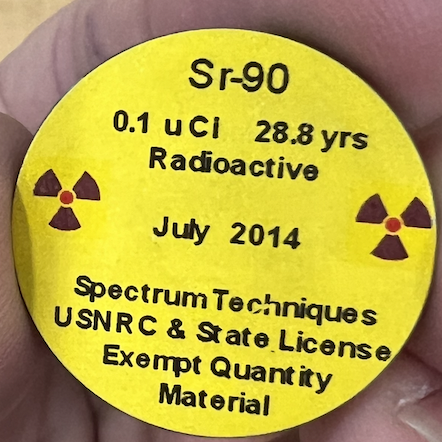
\includegraphics[width=\linewidth]{lab5_a.png}
            
        \end{subfigure}
    \end{minipage}
    \hfill
    \begin{minipage}[t]{0.57\linewidth}
        \centering
        \begin{subfigure}{\linewidth}
            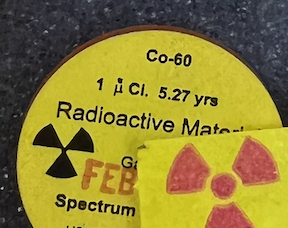
\includegraphics[width=\linewidth]{lab5_b.png}
           
        \end{subfigure}
    \end{minipage}
    \caption{the expected activity of the radioactive sources can be found from the disc labels, and can be converted to $cpm$}
\end{figure}

The background radiation accounted for 39 counts per minute so, we used that to correct the value. The expected counts were found out from the labels, and the efficiency was calculated with the formula provided.

\begin{table}[h!]

  \caption{Data Sheet for GM Tube Efficiency Lab}
  \begin{tabular}{|c|c|c|c|c|}
    \hline
    \textbf{source} & \textbf{Counts} & \textbf{corr. cts} & \textbf{expec. cts} & \textbf{Efficiency (\%)} \\
    \hline
    Sr-90 & 17087 & 17048 & 222000 & 7.7 \\
    \hline
    Co-60 & 984 & 945 & 2220000 & 0.04 \\
    \hline
    Cs-137 & 69636 & 69597 & 1.11E06 & 0.627 \\
    \hline
  \end{tabular}
\end{table}
\subsection*{Note}
As shown in the pictures, the half-lives of the provided isotopes isn't that long, and Co-60 was technically expired. Therefore, such a low value. Same for Sr-90. Cs-137 has a half-life of around 30 years. Nonetheless, the order is the same as predicted/expected. 
\subsection*{Post-Lab Questions}

1. Is the efficiency you calculated for each isotope valid only for that isotope? Explain your answer.\\
\textbf{Answer.} If the conditions while measurements are the same across all isotopes then, yes because there are a lot of factors that can change them. Moreover, it's possible for two isotopes of different elements can have same half-life. \\
\\
2. If a different shelf is used, will the efficiency change? Explain your answer.\\
\textbf{Answer.} The distance also seem to matter. So, yes the efficiency will change. For example, if there is an expanding sphere outside a tunnel. The closer it is to the tunnel, the more of its surface area can penetrate the tunnel. Same analogy can be drawn here. \\
\\
3. The radius of the GM tube’s window is 3.5 cm. The source is 3 cm from the
GM tube. Compare the surface area of a sphere 3 cm from the source to the area of the GM tube’s window. (Hint: find the ratio) How is this related to this experiment? Can this tell you if your results are reasonable?\\
\textbf{Answer.}
\begin{center}
Area=A=$\pi r^2$\\
surface area of sphere having radius 3 cm=$A_s$=$4\pi (3)^2$\\
$A_s$/A=0.34
\end{center}
That explains the huge drop, and seems to be the most significant factor along with half-life and dead-time.
\\

4. (Correlates if five minute and one minute runs were taken.) Are the efficiencies different? How different? Why?\\
\textbf{Answer.} If five minute runs were taken, the efficiency values will be more accurate. Simply because as we've seen there is some randomness associated with radioactivity and it steadies out for longer runs.\\
$$$$


$$$$
%E6

\begin{center}\section*{\underline{Experiment 6: Shelf Ratios}}\end{center}
\subsection*{Introduction}
As mentioned above, not all radiation emitted from our source enters the tube to be counted. It is a function of distance, and the analogy mentioned above is pictured below. It can also be observed the small fraction of the “sphere” that will enter the window of Geiger counter, which is represented by the triangle of sides d and height h.
\begin{figure}[h!]
\centering
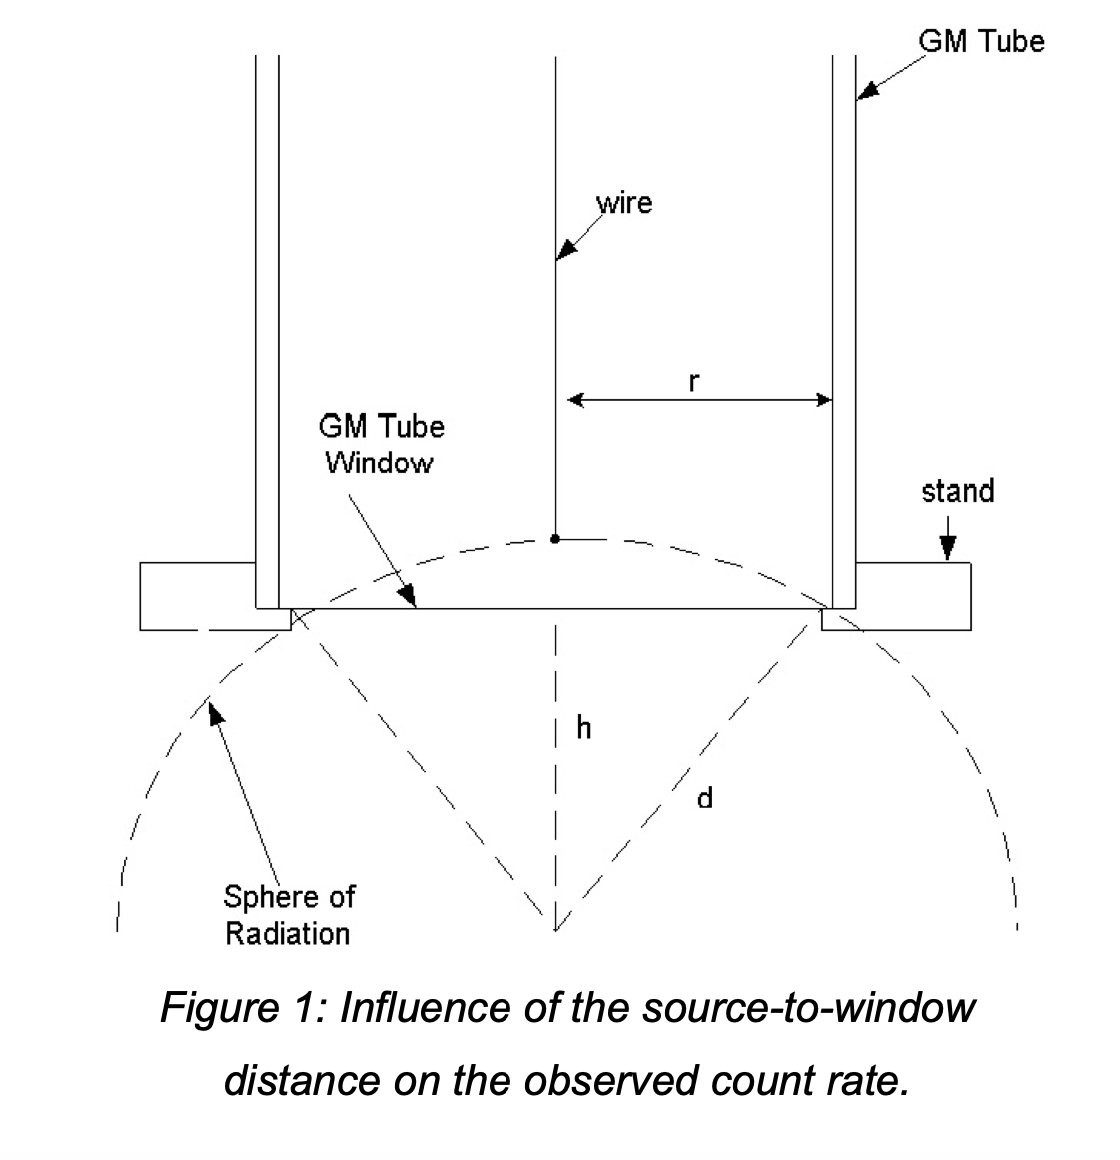
\includegraphics[scale=0.4]{sphere.png}
\caption{The sphere and the tunnel analogy. Not all radiation emitted enters the tube.}
\end{figure}
It follows an inverse square law, and as the source is move moves away, the $beta$ particles will also be attenuated by air molecules, and activity will decrease even more rapidly than predicted by the inverse square law. We'll observe the relationship between distance and activity in this experiment. \\
\subsection*{Pre-Lab Questions}

1. Does radiation gain intensity or lose intensity as a source gets farther from a detector?\\
\textbf{Answer.} Radiation follows inverse square law which states that twice the distance, quarter the intensity. Therefore, intensity drops as a source gets farther from a detector.\\
\\
2. How is radiation emitted from a radioactive source? (Hint: Think of the sun)\\
\textbf{Answer.} The sun undergoes nuclear fusion in its core, and radiation emitted by it is spontaneous due to radioactive decays. Similar to how sun emits radiation due to processes inside its core, radioactive sources emit radiation due to radioactive decays inside the nuclei of their atoms.\\
\\

\subsection*{Procedure}
1. Set-up the counter as before, and voltage to 900V.\\
2. We set the runs to zero and time per run to 30s.\\
3. First, like last time, we do a measurement without any source to measure the background radiation levels.\\
4. Next, we make a measurement with Cs-137 by placing it in the top shelf.\\
5. Next, we lower it down to the second shelf, and take another measurement.\\
5. We keep doing it until we reach the last shelf and have measurements for all shelves.
$$$$
\subsection*{Inference}
The number of counts and shelf ratios dropped significantly as we moved the disc to lower shelves. This can be explained using spherical analogy described above. However, there is an anomaly that it seems to follow $\frac{1}{x}$ more closely than $\frac{1}{x^2}$. There are a couple of possibilities. It could be because the samples were too old. Also, the dead time could be an issue even though we accounted for it. The last but not least, it was observed that the side of the disc mattered. When placed with label side up, the count number was significantly higher than the other side. Even though during this experiment, it was always label-side up but, still we know that it wasn't a perfectly spherical emission of radiation. 
\begin{table}[h!]
  \centering
  \caption{Counts and Distances}
  \begin{tabular}{|c|c|c|c|c|}
    \hline
    \textbf{Shelf\#} & \textbf{cts} & \textbf{Corr. cts} & \textbf{dist. (cm)} & \textbf{Shelf Ratios} \\
    \hline
    1 & 25299 & 25287 & 2 & 1.450 \\
    \hline
    2 & 17449 & 17437 & 4 & 1.000 \\
    \hline
    3 & 12153 & 12141 & 6 & 0.696 \\
    \hline
    4 & 8765 & 8753 & 8 & 0.502 \\
    \hline
    5 & 6344 & 6332 & 10 & 0.363 \\
    \hline
    6 & 4638 & 4626 & 12 & 0.265 \\
    \hline
    7 & 3827 & 3815 & 14 & 0.219 \\
    \hline
    8 & 2947 & 2935 & 16 & 0.168 \\
    \hline
    9 & 2426 & 2414 & 18 & 0.138 \\
    \hline
    10 & 2113 & 2101 & 20 & 0.120 \\
    \hline
  \end{tabular}
  \end{table}

  
\begin{center}
\begin{figure}[h!]
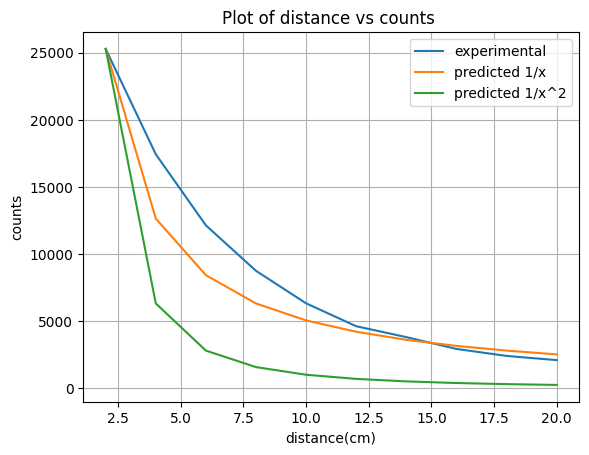
\includegraphics[scale=0.6]{lab6_a.png}
\caption{\small{the count drop significantly as we go to the lower shelves. It was expected that it'll follow inverse square law but, it did not due to the possibilities discussed above.}}
\end{figure}
\begin{figure}[h!]
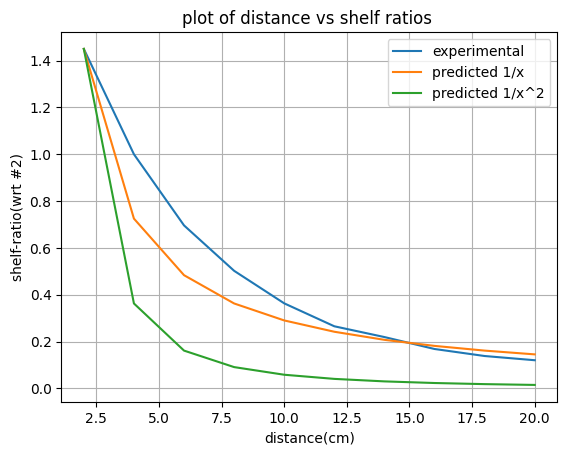
\includegraphics[scale=0.6]{lab6_b.png}
\caption{\small{the shelf ratios drop significantly as we go to the lower shelves. It was expected that it'll follow inverse square law but, it did not due to the possibilities discussed above.}}
\end{figure}
\end{center}

\subsection*{Post-Lab questions}

1. Does the shelf ratio depend on the identity of the sample used?\\
\textbf{Answer.} Yes, it depends but, the general trend should be the same.\\

2. If the experiment is repeated with a gamma or alpha source, what differences
would you expect?\\
\textbf{Answer.} For the gamma source, the count is really high and they can penetrate the air present in the middle more easily than beta, and far more easily than alpha sources. Also, the count difference between shelves will be higher leading to bigger shelf ratio for the first shelf and much smaller for three to ten. However, the general trend should be same(inverse square law).

3. Why is the second shelf the reference shelf?\\
\textbf{Answer.} As we can see when we go to the lower shelves, the count difference between consecutive shelves decreases. Therefore, to get more pronounced measurements in order to find a more distinguishable trend, we start from a lower shelf. We're unsure about the counts before the first shelf because that's where we start. Therefore, we don't choose that as a reference. The second shelf meets this criteria and hence, we choose the second shelf as reference.\\
$$$$

$$$$
%E7

\begin{center}\section*{\underline{Experiment 7: Backscattering}}\end{center}
\subsection*{Introduction}
As we have seen in Rutherford's gold foil experiment, when alpha particles hit a thin gold foil, only some of them pass through others are deflected at angles, and those which are deflected back at 180 $\degree$ are said to be $backscattered$ and this phenomenon in radioactivity is called $backscattering$. In this experiment, we will see the relation between atomic number and backscattering (part I), and for part II, we'll find the relation between thickness and backscattering. In nuclear and particle physics, thickness refers to areal thickness. This is the thickness of the absorbers in $mg/cm^2$.
\begin{center}
\begin{figure}[h!]
\includegraphics[scale=0.25]{bc.png}
\caption{\small{We have used a few of the materials provided, as absorbers in the backscattering experiment.}}
\end{figure}
\end{center}
\subsection*{Pre-Lab Questions}
1. Calculate what percentage of the entire “sphere” surrounding the source does the GM window occupy.\\
\textbf{Answer.} Considering a distance of 3cm and the radius of the GM window be 3.5cm, 34\% as calculated in experiment 5.\\
\\
2. Backscattering does have dependencies on atomic number and on thickness. Does either one dominant the amount of backscattering versus the other? What kind of dependence do you predict for each (direct, inverse, inverse square for example – be descriptive)?\\
\textbf{Answer.} There is expected to be a direct proportionality between both of them and backscattering because the thicker the material or greater the $Z$, there are more interactions between the material and the particles trying to cross it.\\
\subsection*{Procedure}
Part I – Atomic Number Dependence\\
1. As the standard procedure, we set up the geiger counter as before, and set the voltage to 900V.\\
2. Then, we set the runs to zero, and time per run to be 60s.\\
3. We first do a run without a radioactive source to determine the background level.\\ 
4. Next, we place the radioactive source disc at shelf 2, and repeat the measurements.\\
4. Then, we place the absorber directly below it so that the backscattered radiation can be detected by the counter.\\
5. We repeat the above for different materials.\\
Part II – Thickness Dependence\\
1. The first four steps is same as part I.\\
2. Instead of different materials, we want to do measurements for different thicknesses.\\
\subsection*{Inference}
We can use the formula.
\begin{equation*}
\% back=\frac{r-r_0}{r_0}\times 100
\end{equation*}
where  $r $ is the corrected count rate ($cpm$)
and $r_0$ is the count rate without any absorber present.
part I required materials of different atomic numbers. In the kit, we didn't have tin. So the only materials with known atomic numbers were Lead(Pb) and Aluminum(Al). Due to the missing element, we'll use Area thickness as independent variable because it encompasses both Z (usually, greater atomic number means greater density) and thickness.

\begin{table}[h!]
    \centering
    \caption{Material Counts and Thickness}
    \begin{tabular}{|l|l|l|l|}
        \hline
        Material & Corr. Counts & Areal thickness & \% (bc.) \\
        \hline
        Aluminum (Z=13)  & 34607 & 2.82 & 0.6749 \\
        \hline
        Aluminum  & 34531 & 16.4 & 0.4538 \\
        \hline
        Aluminum & 34665 & 65.5 & 0.8436 \\
        \hline
        Aluminum & 34720 & 105 & 1.004 \\
        \hline
        Lead (Z=82)  & 34540 & 431 & 0.48 \\
        \hline
        Lead  & 38305 & 1841.75 & 11.4327 \\
        \hline
        Plastic (Z=N/A)  & 34312 & 4.08 & -0.1833 \\
        \hline
        Background & 45 & & \\
        \hline
        Source & 34420 & & \\
        \hline
    \end{tabular}
\end{table}

\begin{figure}[h!]
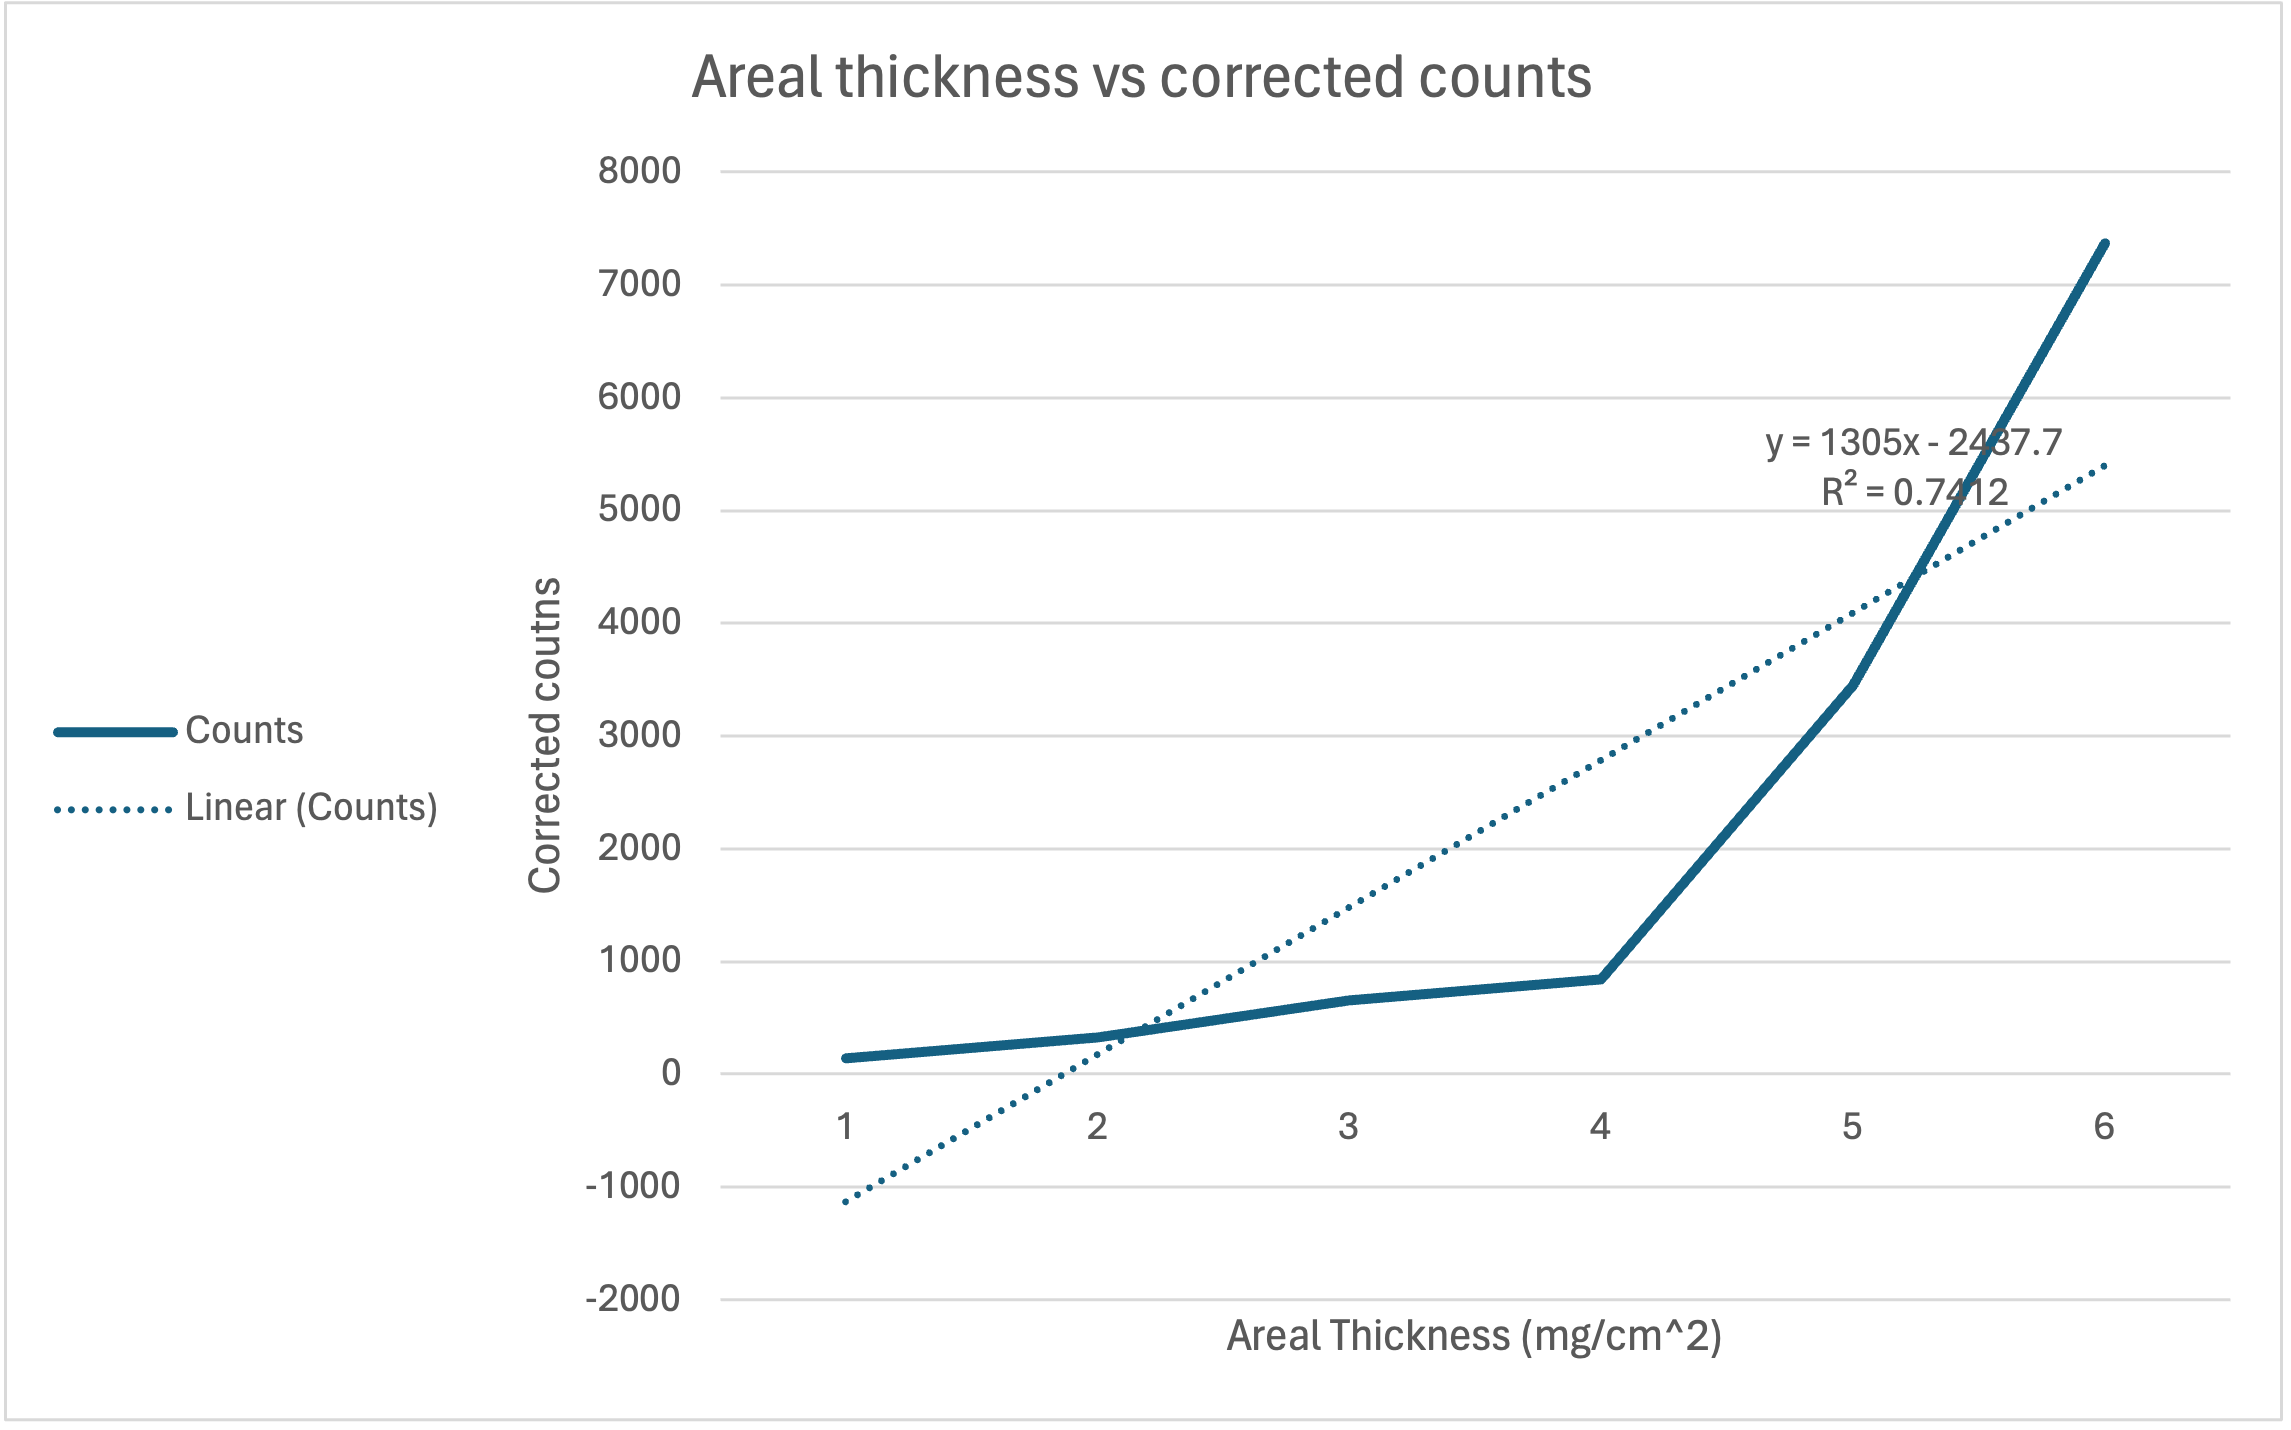
\includegraphics[scale=0.55]{bc_a.png}
\caption{\small{Areal thickness vs corrected counts on a linear scale.}}
\end{figure}

As the Areal thickness increases, count increases because more particles are backscattered which add to the previous particles shooting off directly from the source. Areal thickness is proportional to atomic number and thickness of the material. We can see from the table, as it increases, backscattering increases. For thickness it seems clear. For Z however, we have the thickest lead sample which backscattered the most hinting that it was it's greater atomic number. So, the results are affirmative for both parts, and increasing atomic number or plate thickness will lead to greater backscattering. We have also done the similar experiment by placing the absorber in the middle of the source and the tube. The thickest lead  it has blocked more than 80$\%$ of the counts. \\
\begin{table}[h!]
    \centering
    \caption{Lead as a shield from radiation}
    \begin{tabular}{|c|c|c|}
        \hline
        Thickness (inches) & Areal Thickness & Counts \\
        \hline
        0.064 & 2066 & 1767 \\
        \hline
        0.125 & 3448 & 1436 \\
        \hline
        0.25 & 7367 & 962 \\
        \hline
    \end{tabular}
\end{table}
$$$$
%E13

\begin{center}\section*{\underline{Experiment 13: Half-Life of Ba-137m}}\end{center}
\subsection*{Introduction}
The decay of radioactive atoms occurs at a constant rate therefore, if we know the number of atoms present now, and their decay constant, then we can calculate how many atoms will remain at any future time. 
\begin{equation*}
N(t)=N-\lambda N\Delta t
\end{equation*}
\begin{equation*}
\frac{\Delta N}{\Delta t}=-\lambda N
\end{equation*}
where $N(t)$ is the number of atoms present at time $t$, $\lambda$ is the decay constant, $N$ is the number of atoms present now, $\Delta N=N(t)-N$, and $\Delta t$ is the elapsed time. Another useful term is $half$-$life$. It refers to the time it takes for half the atoms in the original sample to disintegrate. Solving the above equation for continuous time intervals, we find the half-life($t_{1/2}$ as:
\begin{equation*}
t_{1/2}=\frac{ln(2)}{\lambda}
\end{equation*}
\subsection*{Pre-Lab Questions}
1.Explain how you will obtain Ba-137m from the isotope generator.\\
\textbf{Answer.} The source of the Ba-137m is an isotope generator consisting of an exempt quantity of Cs-137 molecules of CsCl. The Ba-137m nuclei are a daughter product that results from the $\lambda$-decay of Cs-137. Ba-137m is separated from the Cs-137 by “milking” the isotope generator.  (spectrum techniques).
\begin{equation*}
{}^{137}_{55}\mathrm{Cs} \rightarrow {}^{137\mathrm{m}}_{56}\mathrm{Ba} + e^{-} + \overline{\nu}_e
\end{equation*}
\\
2. Draw the decay diagram for the process you describe in 1.\\
\textbf{Answer.}
\begin{center}
\begin{figure}[h!]
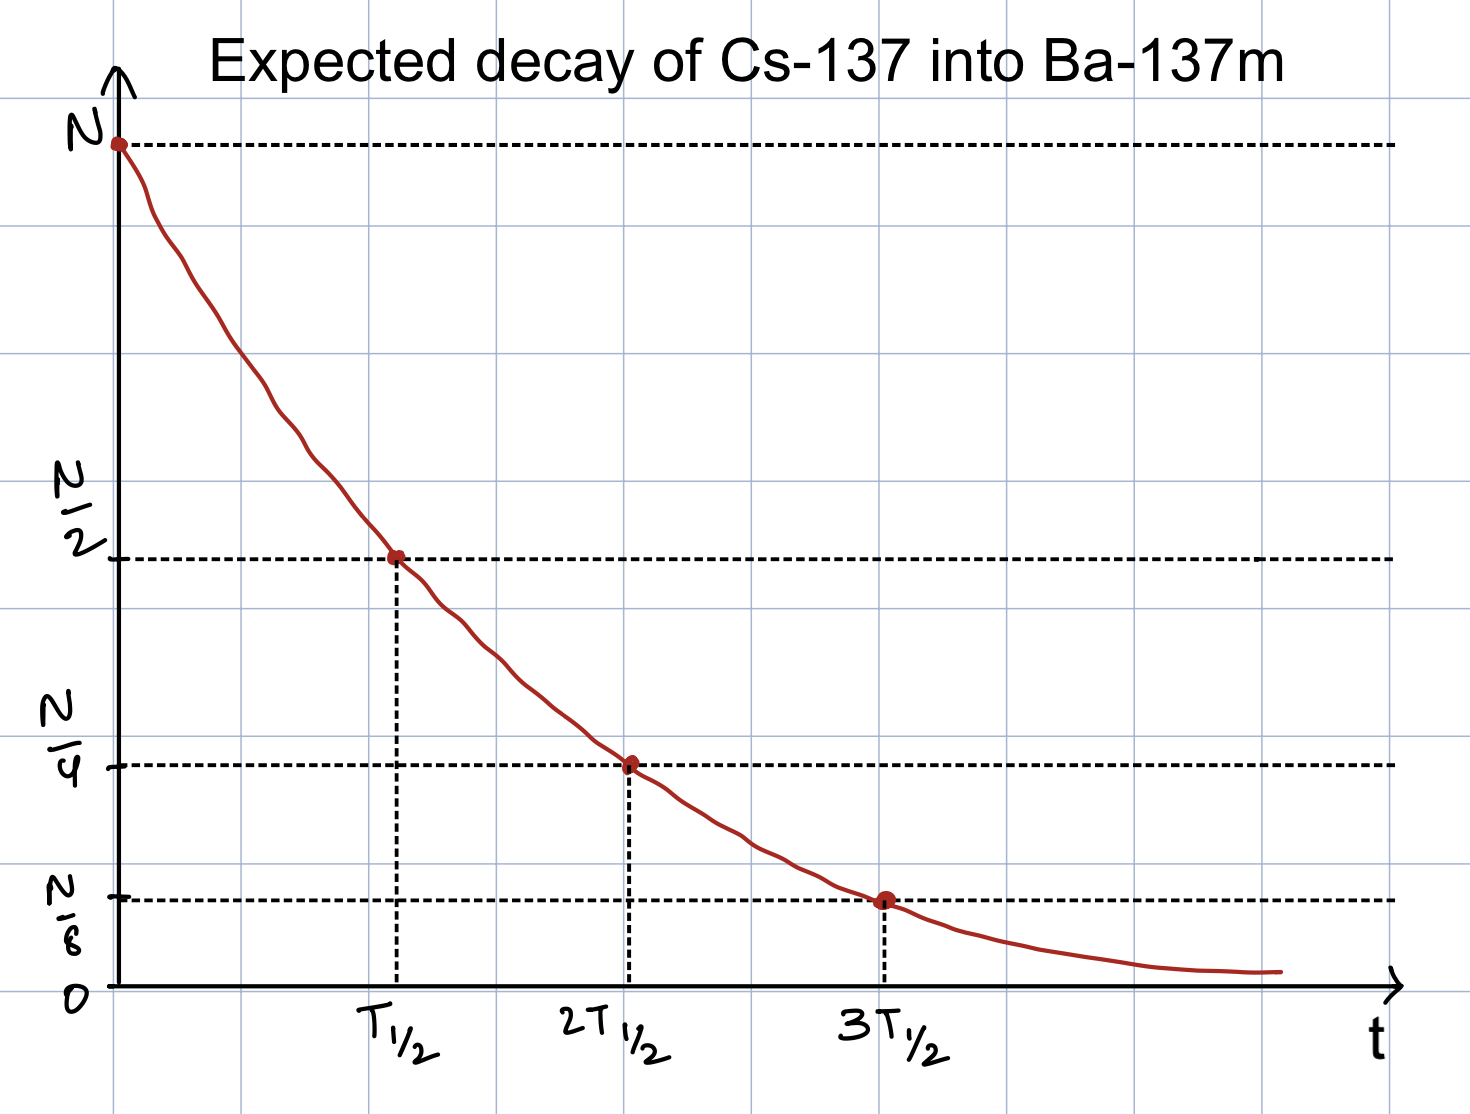
\includegraphics[scale=0.35]{lab13.png}
\caption{\small{decay diagram for the process described in the first question.}}
\end{figure}
\end{center}
3. If a Sr-90 source has a count rate of 7020 $cpm$ today, when will it have a count rate
of 1404 cpm? The half-life of Sr-90 is 28.6 yrs. When will Po-210 reach 1404 cpm
from 7020 cpm (half-life for Po-210 is 138 days)?\\
\textbf{Answer.}
\begin{equation*}
N(t)=N_02^{-\frac{t}{t_{1/2}}}
\end{equation*}
because $cpm$ is proportional to the number of atoms present at time t, and we don't need to convert it to years. We can write it as it is.
\begin{equation*}
\frac{1}{5}=2^{-\frac{t}{28.6}}\implies t=66.4 yrs
\end{equation*}
Similarly, solvinfgfor Po-210, we get, 320.4 days.\\

4. If a Tl-204 source has 1.34E21 atoms today. When will it have 1.675E18
atoms? The half-life for Tl-204 is 3.78 years.\\
\textbf{Answer.}
\begin{equation*}
\frac{ln{\frac{1.675E18}{1.34E21}}}{ln(2)}=\frac{-t}{t_{1/2}}\implies t=36.45 yrs
\end{equation*}
\subsection*{Procedure}
1. We set-up the counter as before, and set the set the voltage to 900V.\\
2. Next, we set the runs to zero, and time per run to 30s.\\
3. Like before, first we do measurements without anything to determine the background radiation.\\
4. From the isotope generator, we obtain 10-12 drops of Ba-137m with a needleless syringe, and put them into a small plate. After that, we put it into the shelf.\\
5. Finally, we do 31 runs with 30s each, and save the data.
\subsection*{Inference}
The sample decays pretty quickly, much more than all previous samples.
\begin{center}
\begin{figure}[h!]
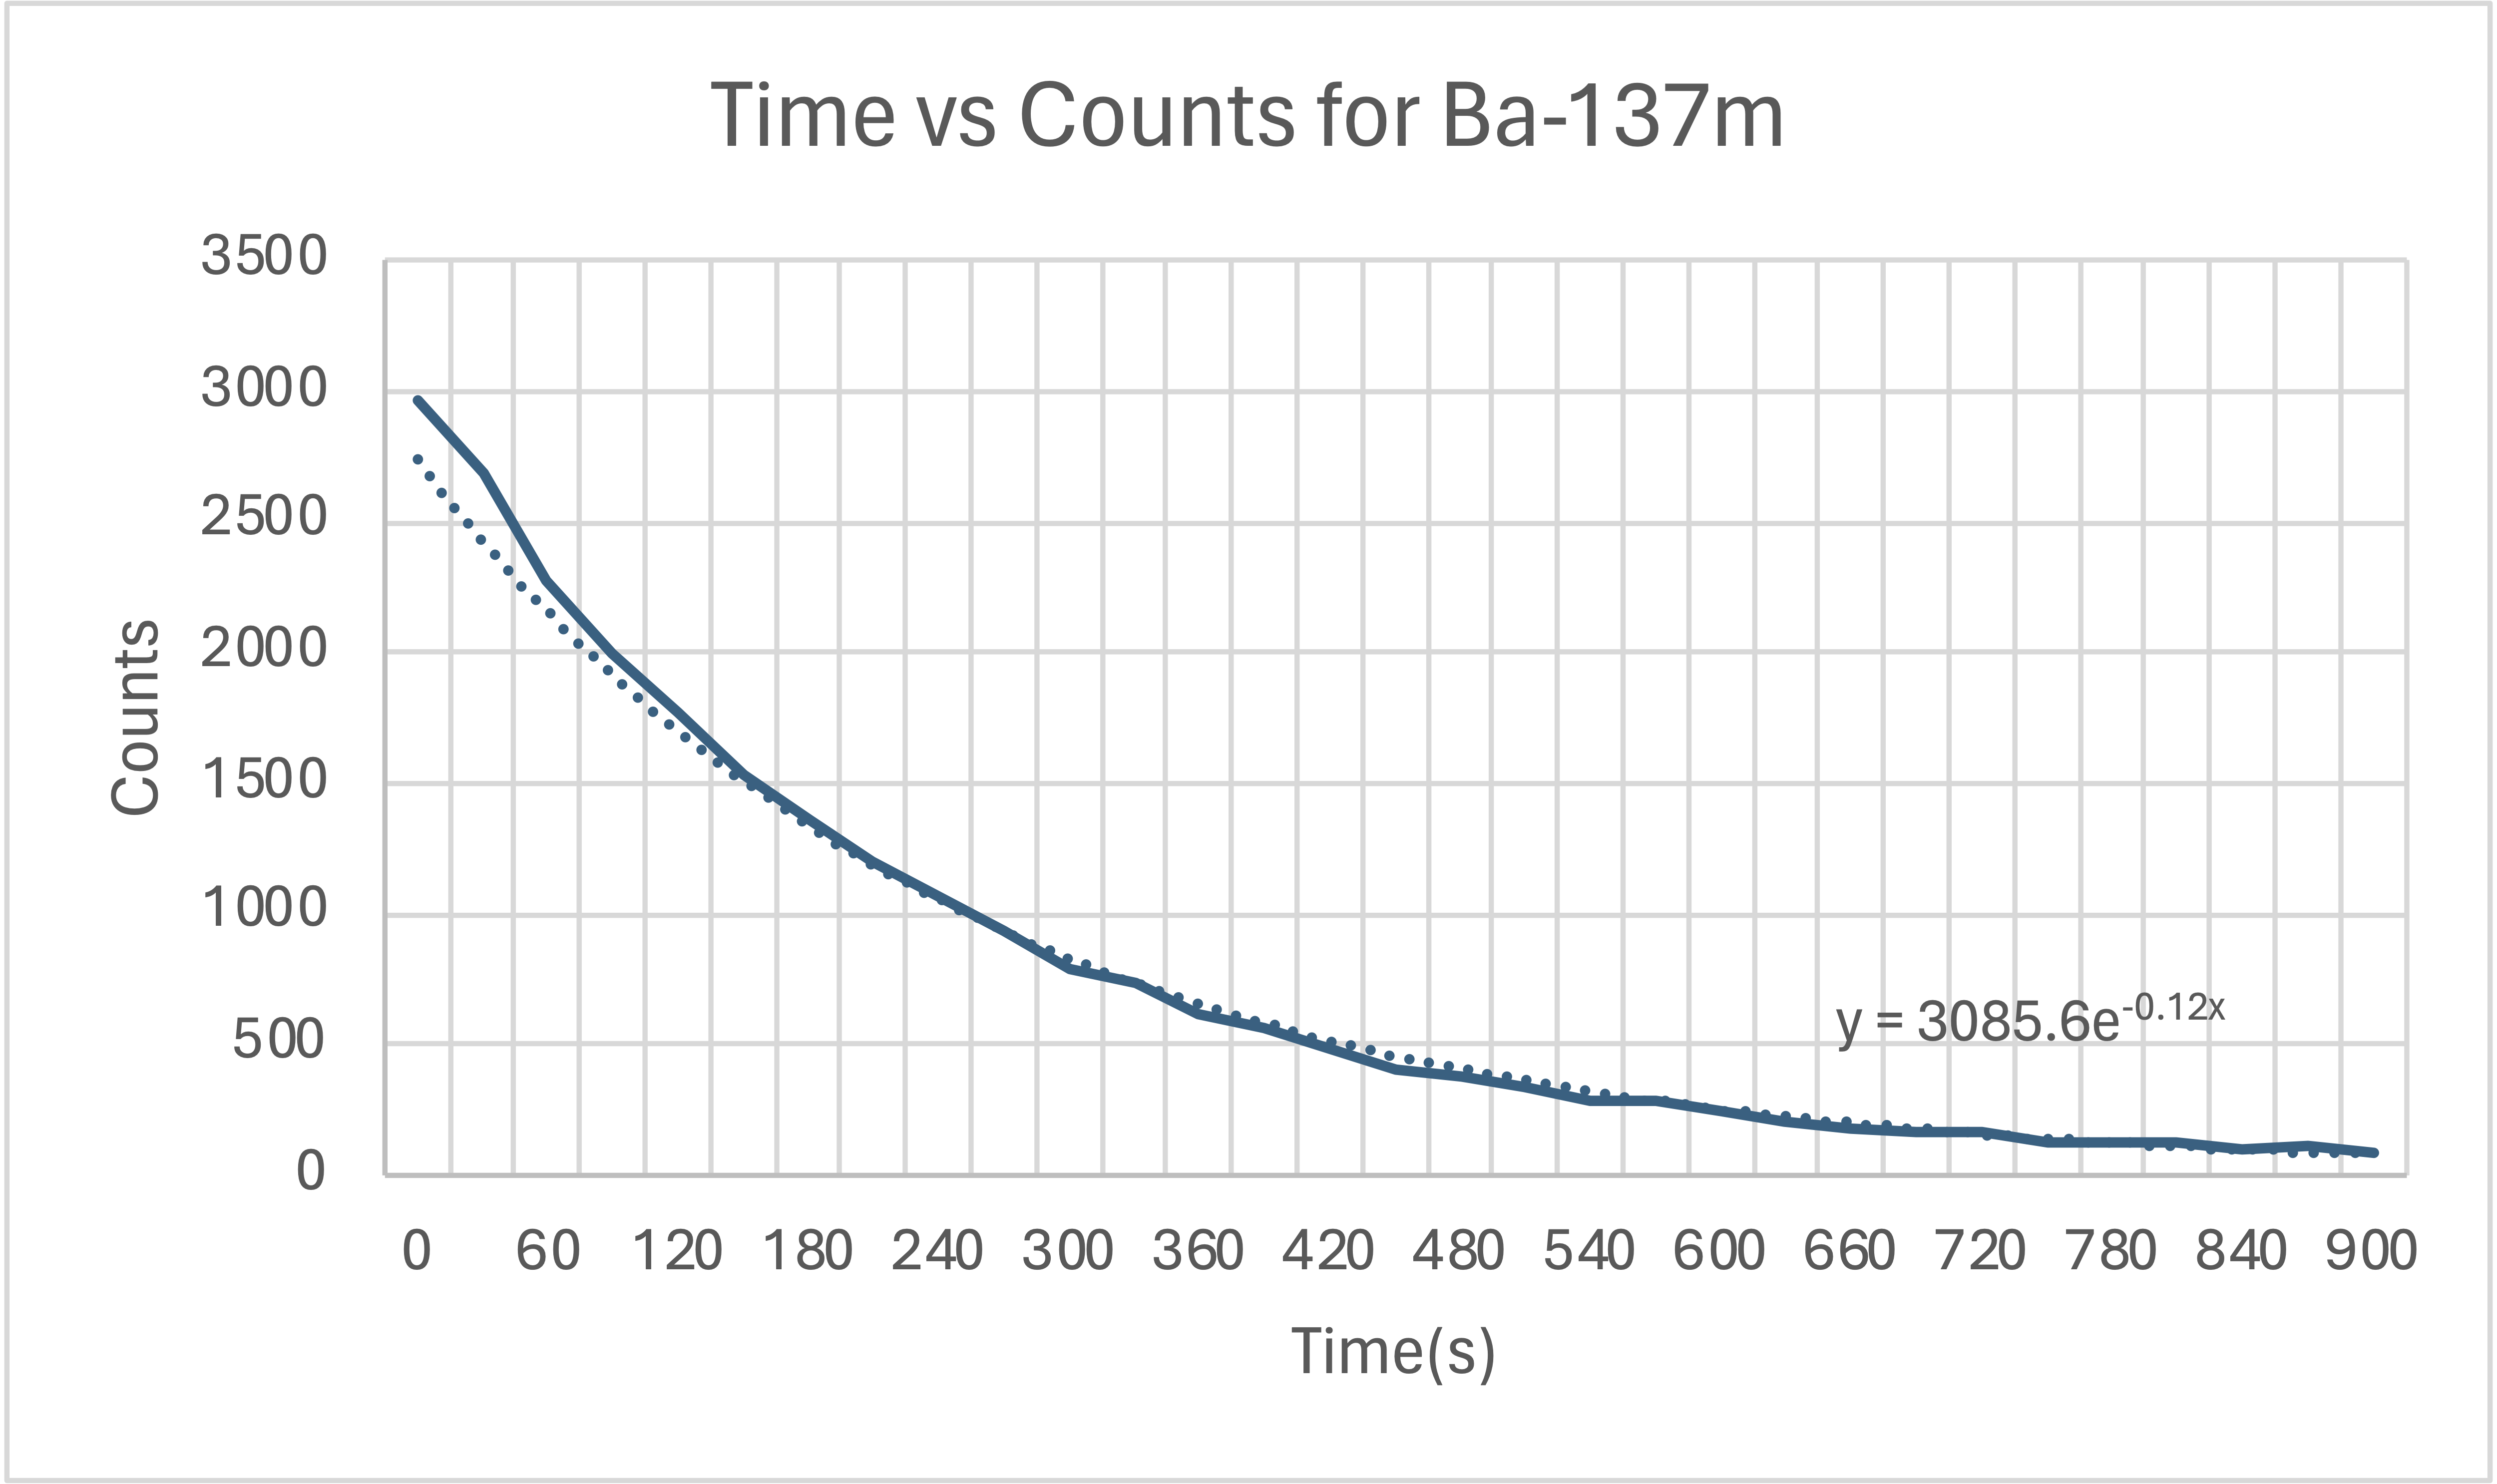
\includegraphics[scale=0.055]{lab13_b.png}
\caption{\small{The half-life of Ba-137m is very small compared to Cs-137, and other samples previously used. We can also see from the fitted equation, the decay constant is around 0.12. }}
\end{figure}

\begin{figure}[h!]
\centering
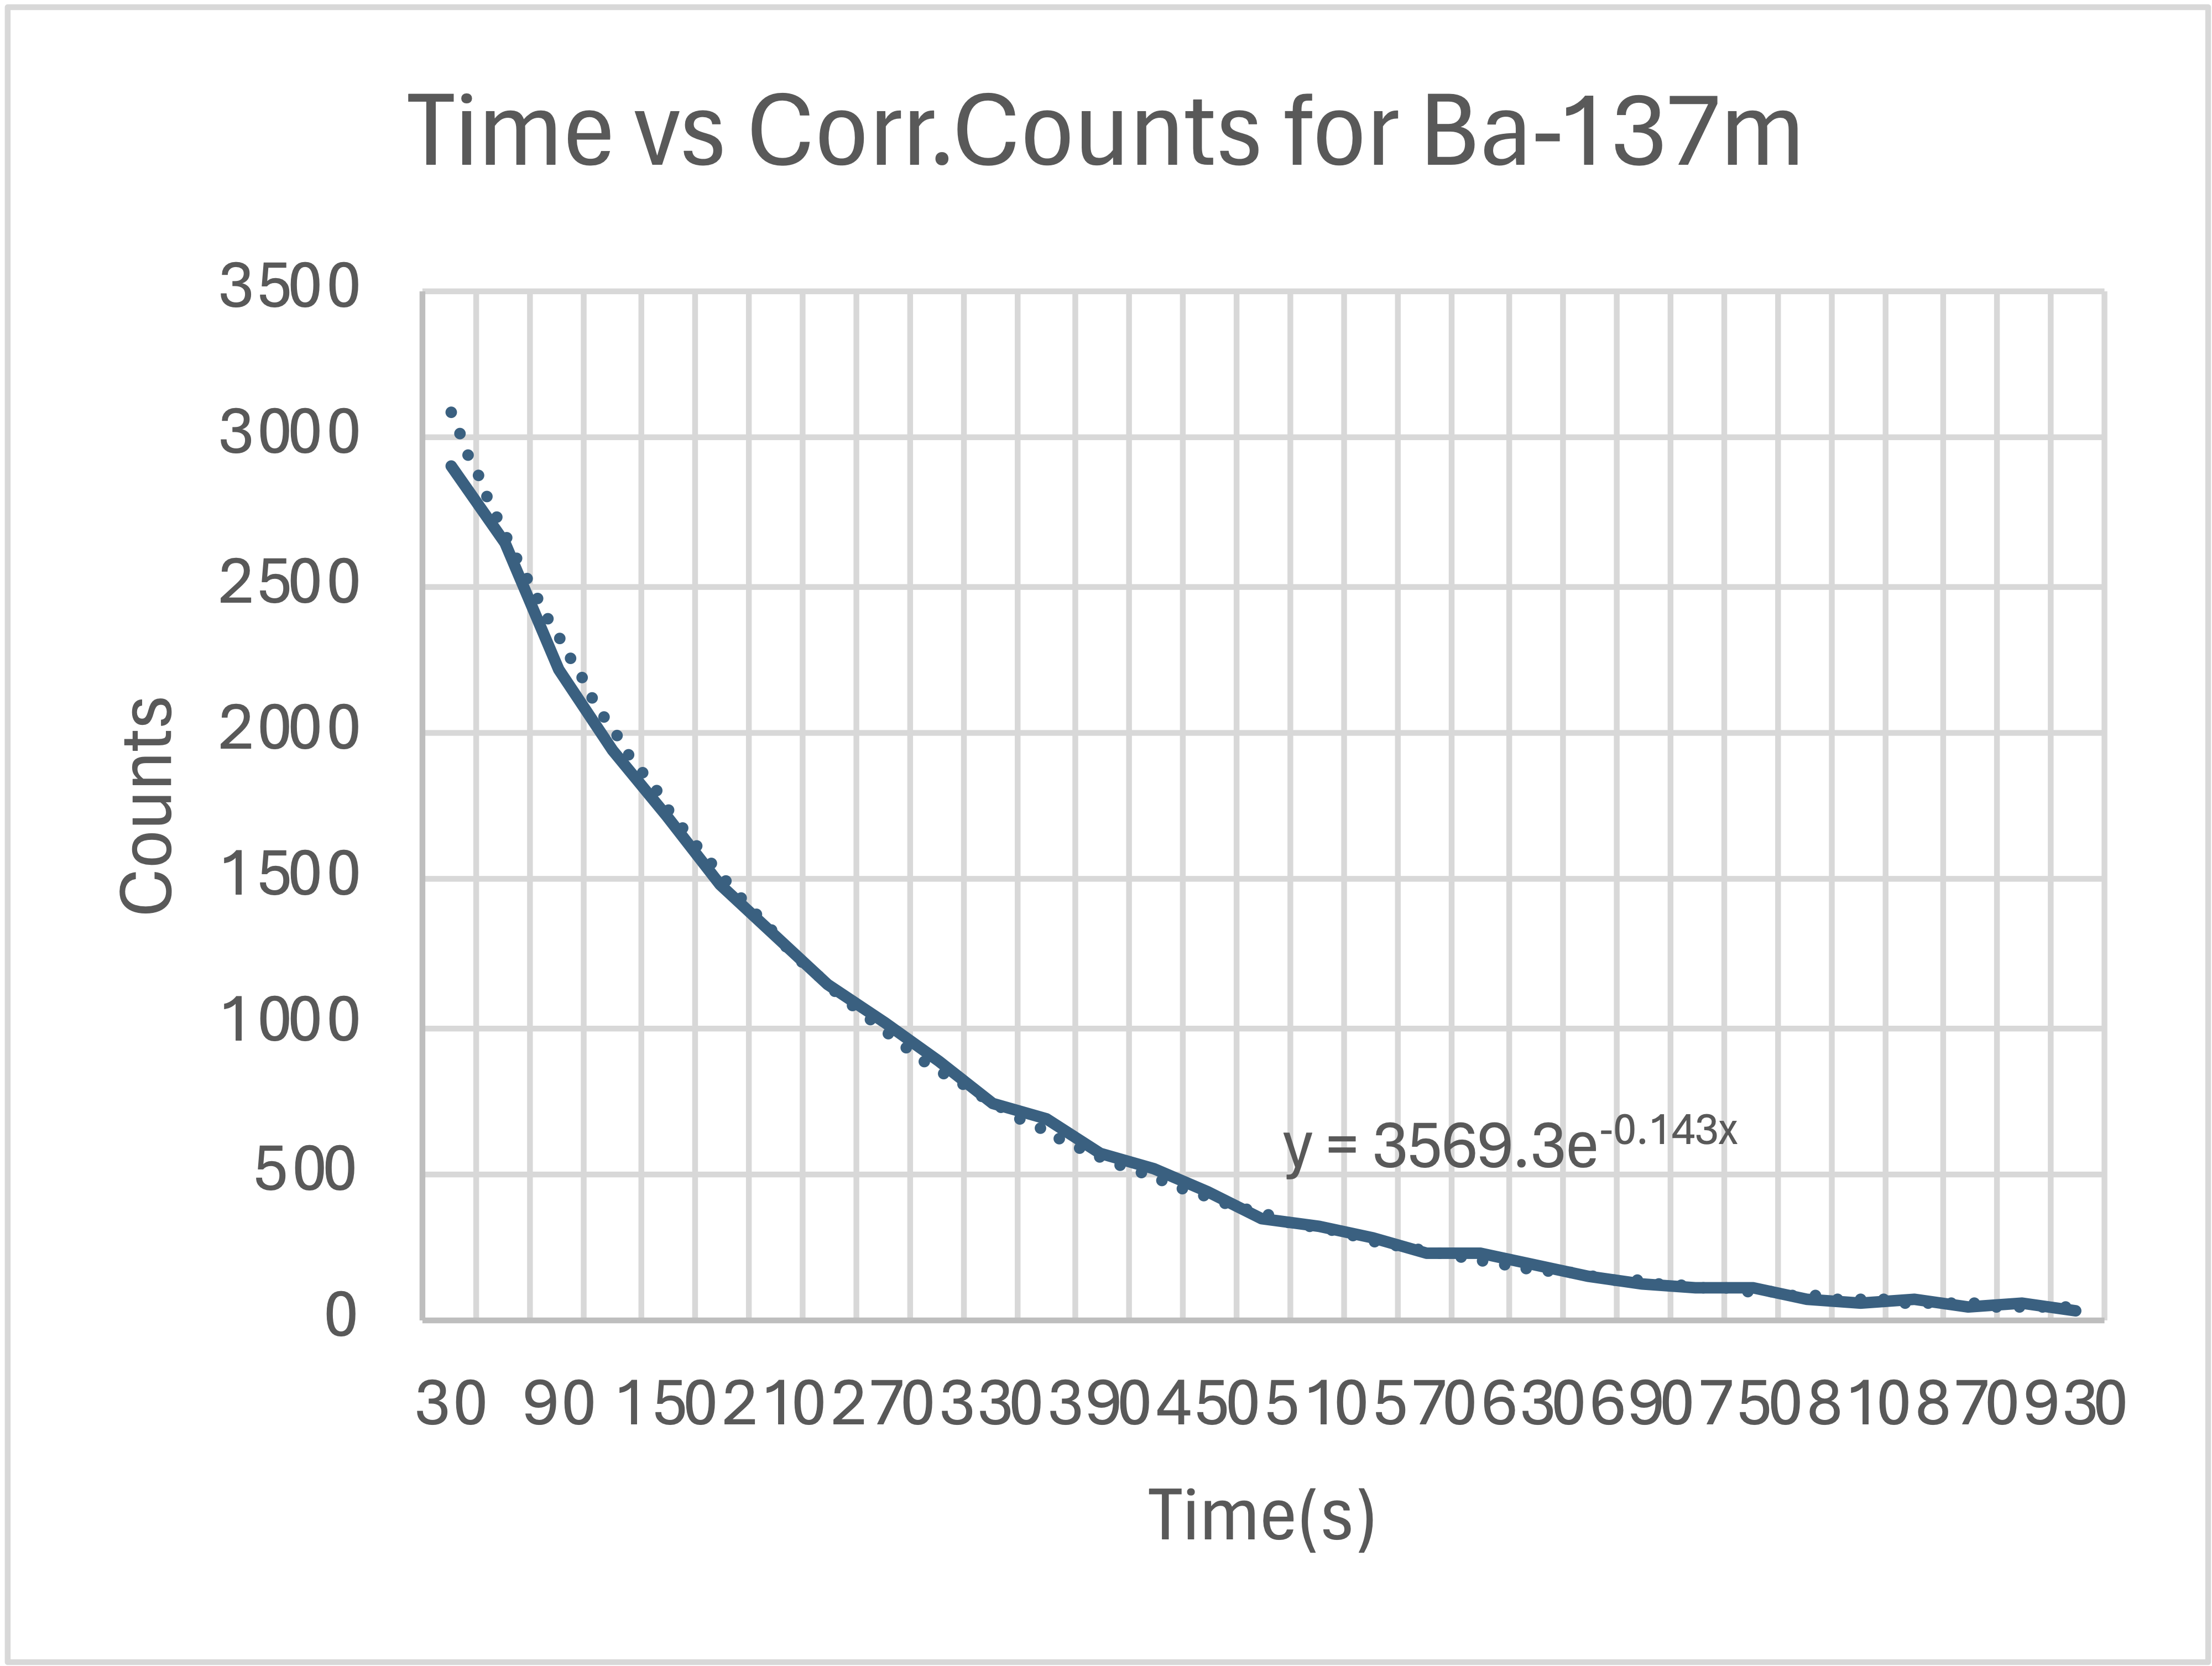
\includegraphics[scale=0.065]{lab13_c.png}
\caption{\small{ representation of time(s) vs corrected counts }}
\end{figure}
\begin{figure}[h!]
\centering
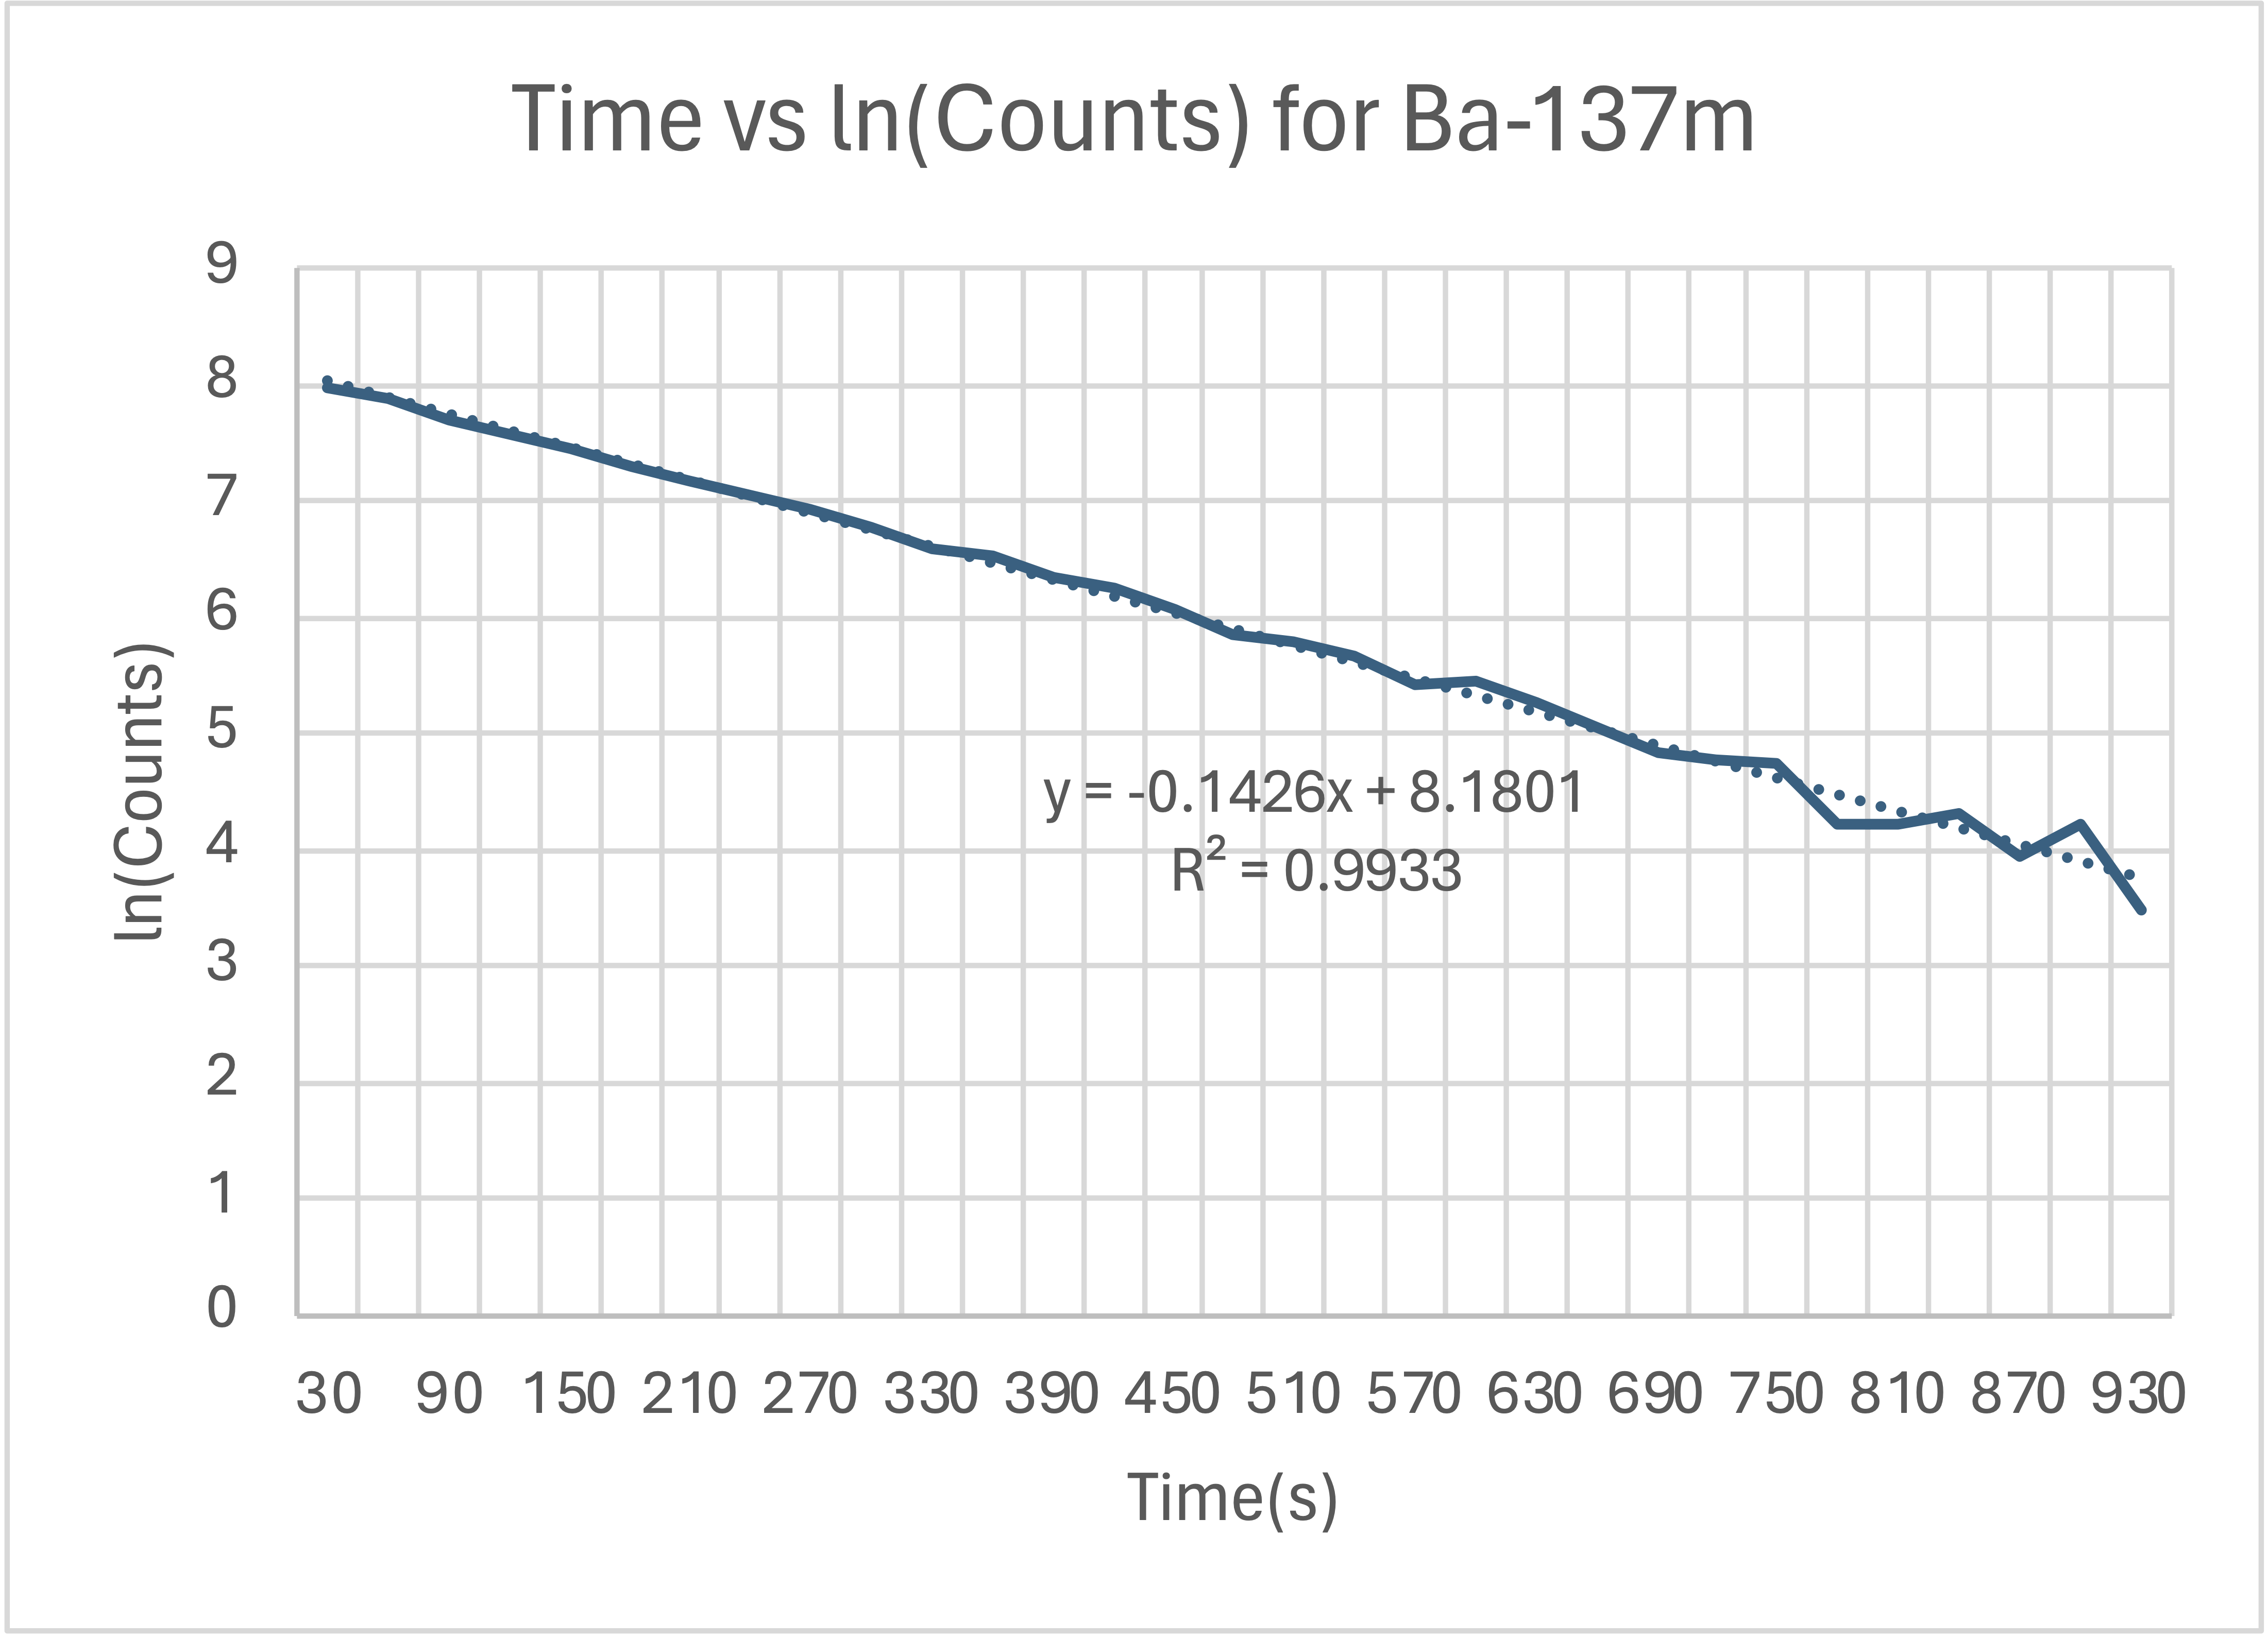
\includegraphics[scale=0.06]{lab13_d.png}
\caption{\small{logarithmic(natural) representation of time vs corrected counts }}
\end{figure}
\end{center}


\begin{table}[h!]
\small
\caption{Conclusions:}
\begin{tabular}{|l|l|l|l|l|}
\hline
Data Points & $\lambda$ & $t_{1/2}$ (s) & Error & \# of $\sigma$'s \\
\hline
first half & 0.004507514 & 153.7759 & 3.72307E-05 & 0.113488233 \\
\hline
second half & 0.004904668 & 141.324 & 0.000270593 & 2.022013571 \\
\hline
All & 0.004752838 & 145.8386 & 7.25377E-05 & 1.164594443 \\ 
\hline
\end{tabular}
\end{table}

$$$$


\begin{table}[h!]
\centering
\caption{Data Sheet for Half-Life Lab}
\begin{tabular}{|l|l|l|l|l|}
\hline
Counts & Corr.Counts & ln(Counts) & Time(s) \\
\hline
2961 & 2911 & 7.976251944 & 30 \\
\hline
2691 & 2641 & 7.878912912 & 60 \\
\hline
2269 & 2219 & 7.704811923 & 90 \\
\hline
1992 & 1942 & 7.571473649 & 120 \\
\hline
1769 & 1719 & 7.449498005 & 150 \\
\hline
1532 & 1482 & 7.301147806 & 180 \\
\hline
1363 & 1313 & 7.180069874 & 210 \\
\hline
1198 & 1148 & 7.045776577 & 240 \\
\hline
1066 & 1016 & 6.923628628 & 270 \\
\hline
940 & 890 & 6.791221463 & 300 \\
\hline
789 & 739 & 6.605297921 & 330 \\
\hline
734 & 684 & 6.527957918 & 360 \\
\hline
618 & 568 & 6.342121419 & 390 \\
\hline
565 & 515 & 6.244166901 & 420 \\
\hline
488 & 438 & 6.08221891 & 450 \\
\hline
400 & 350 & 5.857933154 & 480 \\
\hline
375 & 325 & 5.783825182 & 510 \\
\hline
339 & 289 & 5.666426688 & 540 \\
\hline
279 & 229 & 5.433722004 & 570 \\
\hline
281 & 231 & 5.442417711 & 600 \\
\hline
244 & 194 & 5.267858159 & 630 \\
\hline
207 & 157 & 5.056245805 & 660 \\
\hline
174 & 124 & 4.820281566 & 690 \\
\hline
169 & 119 & 4.779123493 & 720 \\
\hline
164 & 114 & 4.736198448 & 750 \\
\hline
119 & 69 & 4.234106505 & 780 \\
\hline
118 & 68 & 4.219507705 & 810 \\
\hline
125 & 75 & 4.317488114 & 840 \\
\hline
102 & 52 & 3.951243719 & 870 \\
\hline
117 & 67 & 4.204692619 & 900 \\
\hline
82 & 32 & 3.465735903 & 930 \\
\bottomrule
\end{tabular}
\end{table}
\newpage 
\href{https://github.com/fnuArsh/Radioactivity_lab}{click here for lab files.}\\
\href{https://colab.research.google.com/drive/1xOXSxfqtyZU8cyClQZAxoPkxcLuAKhI2?usp=sharing}{click here for basic colab code used.}



\end{document}  